% Initial version by Darian Muresan, Ph.D.
% dmuresan@stevens.edu
% Edit and adjust as needed.
\documentclass[12pt]{cornell}

% add index support
%\usepackage{imakeidx}
\usepackage{makeidx}
%\makeindex

% graphing programs
\usepackage{color}
\usepackage{psfrag}
\usepackage{verbatim}
\usepackage{fancyhdr}
%\usepackage{titlesec}
\usepackage{fancyvrb} 
% hyperlink programs
%\usepackage{url}

% Does not work with LaTeX=>PDF
\usepackage[pdfmark, 
breaklinks=true, 
colorlinks=true,
citecolor=blue,
linkcolor=blue,
menucolor=black,
pagecolor=black,
urlcolor=blue
]{hyperref} % links in pdf

%\usepackage[colorlinks]{hyperref} % links in dvi
\usepackage{listings}
\usepackage{amsfonts} 
\usepackage{amssymb} 
%\usepackage{tabto}

\usepackage{tabularx,colortbl}
\usepackage[chapter]{algorithm} 
\usepackage{algorithmic} 
\usepackage{blindtext}

\definecolor{DarkGreen}{rgb}{0,0.6,0}
\definecolor{mygreen}{rgb}{0,0.6,0}
\definecolor{mygray}{rgb}{0.5,0.5,0.5}
\definecolor{mymauve}{rgb}{0.58,0,0.82}

\usepackage{tocloft}
\usepackage{amsmath}
\usepackage{tcolorbox}
\usepackage{enumitem}
\usepackage{longtable}
%\usepackage{textcomp}
\usepackage{txfonts}
\usepackage{pstool}

%part for \part titles
%chap for \chapter titles
%sec for \section titles
%subsec for \subsection titles
%subsubsec for \subsubsection titles
%para for \paragraph titles
%subpara for \subparagraph titles
%fig for figure \caption titles
%subfig for subfigure \caption titles
%tab for table \caption titles
%subtab for subtable \caption titles


% update chapter number spacing
\setlength{\cftchapnumwidth}{2em}
\setlength{\cftsecnumwidth}{2.5em}
\setlength{\cftsubsecnumwidth}{3.5em}
\setlength{\cftsubsubsecnumwidth}{4.5em}

\addtolength{\cftsecindent}{0.5em}
\addtolength{\cftsubsecindent}{0.5em}
\addtolength{\cftsubsubsecindent}{0.5em}

%\titlespacing*{\chapter}{0pt}{-50pt}{20pt}
%\titleformat{\chapter}[display]{\normalfont\huge\bfseries}{\chaptertitlename\ 
%\thechapter}{20pt}{\Huge}
%\pagestyle{fancy}
%\pagestyle{cornell}
%
%\rhead{F054-021-0172}
%\chead{Nonlinear Enhancement of Visual Target Detection (AF05-T021)}
%\lhead{GSTI}
%\lfoot{\scriptsize Use or disclosure of data on this page is subject
%to the restriction on the title page of this proposal.}
%\cfoot{}
%\rfoot{\thepage}

\newfont{\Bp}{msbm10}
\newfont{\BpBig}{msbm10 scaled\magstep2}
\newfont{\Sc}{eusm10}
\newfont{\ScBig}{eusm10 scaled\magstep3}
\newfont{\Fr}{eufm10}
\newfont{\FrBig}{eufm10 scaled\magstep1}

% some commands:
\newcommand{\dxi}{{\tt m\_xDeltaInput}}
\newcommand{\dyi}{{\tt m\_yDeltaInput}}
\newcommand{\dci}{{\tt m\_cDeltaInput}}
\newcommand{\dxo}{{\tt m\_xDeltaOutput}}
\newcommand{\dyo}{{\tt m\_yDeltaOutput}}
\newcommand{\dco}{{\tt m\_cDeltaOutput}}
\newcommand{\ttf}[1]{{\tt #1}}
\newcommand{\tbl}[2]{{\begin{tabular}{c} #1 \\ #2 \end{tabular}}}

\newcommand{\urltwo}[2]{\mbox{\href{#1}{\tt #2}}}
\newcommand{\qnorm}[1]{\|#1\|_{\bQ}}
\newcommand{\qdot}[2]{\lrb #1, #2 \rrb_{\bQ}}
\newcommand{\kdot}[2]{\lrb #1, #2 \rrb_{\bf k}}
\newcommand{\tdot}[2]{\lrb #1, #2 \rrb}
\newcommand{\mydiff}[2]{\lrb #1 - #2 \rrb}
\newcommand{\lena}{\textit{lena}}
\newcommand{\barb}{\textit{barbara}}
\newcommand{\boat}{\textit{boat}}
\newcommand{\leaves}{\textit{leaves}}
\newcommand{\rings}{\textit{rings}}
\newcommand{\treg}{\textit{train region}}
\newcommand{\dreg}{\textit{denoise region}}
\newcommand{\oreg}{\textit{overlap region}}
\newcommand{\sil}{\sigma_l^2}
\newcommand{\sn}{\sigma^2}
\newcommand{\bn}{{\mbox{\bf \FrBig N}}}
\newcommand{\n}{\mbox{\Fr N}}
%\newcommand{\bn}{\bf N}
%\newcommand{\n}{N}
\newcommand{\bY}{\textbf{Y}}
\newcommand{\bX}{\textbf{X}}
\newcommand{\bb}{\textbf{b}}
\newcommand{\bu}{\textbf{u}}
\newcommand{\bv}{\textbf{v}}
\newcommand{\by}{\textbf{y}}
\newcommand{\bx}{\textbf{x}}
\newcommand{\be}{\textbf{e}}
\newcommand{\bz}{\textbf{z}}
\newcommand{\bs}{\textbf{s}}
\newcommand{\bw}{\textbf{w}}
\newcommand{\bQ}{\textbf{Q}}
\newcommand{\bphi}{\textbf{$\phi$}}
\newcommand{\lsb}{\left[}
\newcommand{\rsb}{\right]}
\newcommand{\lrb}{\left(}
\newcommand{\rrb}{\right)}
\newcommand{\lcb}{\left\{}
\newcommand{\rcb}{\right\}}
\newcommand{\R}{\mbox{\BpBig R}}
\newcommand{\F}{{\cal F}}
\newcommand{\Fk}{\mbox{\Sc F}}
\newcommand{\bQF}{\textbf{Q}_{\mbox{\Sc F}}}
\newcommand{\N}{{\cal N}}
\newcommand{\xlz}{X_l(z)}
\newcommand{\xhz}{X_h(z)}
\newcommand{\xz}{X(z)}
\newcommand{\pr}{ perfect reconstruction }
\newcommand{\smb}{Smith-Barnwell }
\newcommand{\xw}{X(e^{j\omega})}
\newcommand{\xmw}{X(-e^{j\omega})}
\newcommand{\dw}{D(e^{j\omega})}
\newcommand{\dmw}{D(-e^{j\omega})}
\newcommand{\ew}{E(e^{j\omega})}
\newcommand{\emw}{E(-e^{j\omega})}
\newcommand{\fw}{F_0(e^{j\omega})}
\newcommand{\fmw}{F_0(-e^{j\omega})}
\newcommand{\hoz}{H_1(z)}
\newcommand{\hzz}{H_0(z)}
\newcommand{\goz}{G_1(z)}
\newcommand{\gzz}{G_0(z)}
\newcommand{\hzw}{H_{0}(e^{j\omega})}
\newcommand{\hzmw}{H_{0}(-e^{j\omega})}
\newcommand{\hzcw}{H_{0}(e^{-j\omega})}
\newcommand{\how}{H_1(e^{j\omega})}
\newcommand{\homw}{H_1(-e^{j\omega})}
\newcommand{\gzw}{G_0(e^{j\omega})}
\newcommand{\gzmw}{G_0(-e^{j\omega})}
\newcommand{\gow}{G_1(e^{j\omega})}
\newcommand{\gomw}{G_1(-e^{j\omega})}
\newcommand{\wl}{e^{-jwL}}
\newcommand{\aqua}{\textit{AQua with OR }}
\newtheorem{theorem}{Theorem}
\newtheorem{lemma}{Lemma}
\newtheorem{corollary}{Corollary}
\newtheorem{claim}{Claim}
\newtheorem{definition}{Definition}
\newenvironment{proof}{\noindent{\em Proof.}}{\ \hfill Q.E.D.}
%\newtheorem{moduleCount}{L}
\newcommand*{\labelfile}[1]{%
  \label{file:#1}%
}

% Use this to label requirements, use cases, user stories, etc.
% This is where we can add different spellings for different types of 
% requirements, use cases, user stories, etc.
% \newtheorem{requirementKind}{Requirement Spelling}
\newtheorem{reqkFunctional}{Functional Requirement}
\newtheorem{reqkQuality}{Quality Requirement}
\newtheorem{reqkConstraint}{Constraint Requirement}
\newtheorem{reqkInterface}{Interface Requirement}
\newtheorem{reqkBusiness}{Business Requirement}
% Use cases
\newtheorem{useCase}{Use Case}
% User story
\newtheorem{userStory}{User Story}

% command for adding a version to the document
\newcommand{\VERSION}{Version 0.0.0}

% Family -- enter the name of the family that it belongs to: Chapter, Figure, Table, etc.
% Name -- name of the family member: file name, table name, etc.
\newcommand{\FamilyName}[2]{\hyperref[#1::#2]{#2}\index{#2}\xspace}
% Family -- same as above
% Name -- same as above
% Reference -- shorthand for the 'Name'.  It will show as Reference_NameID
% Kind -- underscore(_), space, or dash (-)
\newcommand{\FamilyNameReferenceKind}[4]{\hyperref[#1::#2]{$#3#4{\ref*{#1::#2}}$}}
% newcommand{Family,Label}
\newcommand{\FamilyLabel}[2]{\label{#1::#2}}


% for use cases
\newcommand{\UseCaseLabel}[1]{\FamilyLabel{UseCase}{#1}}
\newcommand{\UseCaseName}[1]{\FamilyName{UseCase}{#1}}
\newcommand{\UseCaseReference}[1]{\FamilyNameReferenceKind{UseCase}{#1}{UC}{_}}
% UseCase name with stacked reference
\newcommand{\UseCaseNameWSReference}[1]{\begin{tabular}{c}\UseCaseName{#1} \\ (\UseCaseReference{#1}) \end{tabular}}
% UseCase name with inline reference
\newcommand{\UseCaseNameWIReference}[1]{\UseCaseName{#1} (\UseCaseReference{#1})}

% for chapters
\newcommand{\ChapterName}[1]{\FamilyName{Chapter}{#1}}
\newcommand{\ChapterLabel}[1]{\FamilyLabel{Chapter}{#1}}
\newcommand{\ChapterReference}[1]{\FamilyNameReferenceKind{Chapter}{#1}{Chapter}{\mbox{ }}}
% Chapter name with inline (WI) reference 
\newcommand{\ChapterNameWIReference}[1]{\ChapterName{#1} (\ChapterReference{#1})}

% for figures
\newcommand{\FigureName}[1]{\FamilyName{Figure}{#1}}
\newcommand{\FigureLabel}[1]{\FamilyLabel{Figure}{#1}}
\newcommand{\FigureReference}[1]{\FamilyNameReferenceKind{Figure}{#1}{Figure}{\mbox{ }}}
% Figure name with stacked (WS) reference
\newcommand{\FigureNameWSReference}[1]{\begin{tabular}{c}\FigureName{#1} \\ (\FigureReference{#1}) \end{tabular}}
% Figure name with inline (WI) reference 
\newcommand{\FigureNameWIReference}[1]{\FigureName{#1} (\FigureReference{#1})}

% for tables
\newcommand{\TableName}[1]{\FamilyName{Table}{#1}}
\newcommand{\TableLabel}[1]{\FamilyLabel{Table}{#1}}
\newcommand{\TableReference}[1]{\FamilyNameReferenceKind{Table}{#1}{Table}{\mbox{ }}}

% for requirements
% RequirementLabel[Kind][Label]
\newcommand{\RequirementLabel}[2]{\FamilyLabel{#1}{#2}}
\newcommand{\RequirementName}[2]{\FamilyName{#1}{#2}}
\newcommand{\RequirementReference}[2]{\FamilyNameReferenceKind{#1}{#2}{#1}{_}}
% Requirements name with stacked (WS) reference
\newcommand{\RequirementNameWSReference}[2]{\begin{tabular}{c}\RequirementName{#1}{#2} \\ (\RequirementReference{#1}{#2}) \end{tabular}}
% Requirements name with inline (WI) reference 
\newcommand{\RequirementNameWIReference}[2]{\RequirementName{#1}{#1} (\RequirementReference{#1}{#2})}

% for requirements
% RequirementLabel[Kind][Label]
\newcommand{\UserStoryLabel}[2]{\FamilyLabel{#1}{#2}}
\newcommand{\UserStoryName}[2]{\FamilyName{#1}{#2}}
\newcommand{\UserStoryReference}[2]{\FamilyNameReferenceKind{#1}{#2}{R}{_}}
% Requirements name with stacked (WS) reference
\newcommand{\UserStoryNameWSReference}[2]{\begin{tabular}{c}\RequirementName{#1}{#2} \\ (\RequirementReference{#1}{#2}) \end{tabular}}
% Requirements name with inline (WI) reference 
\newcommand{\UserStoryNameWIReference}[2]{\RequirementName{#1}{#1} (\RequirementReference{#1}{#2})}



\lstset{ %
  backgroundcolor=\color{white},   % choose the background color; you must add \usepackage{color} or \usepackage{xcolor}
  basicstyle=\footnotesize,        % the size of the fonts that are used for the code
  breakatwhitespace=false,         % sets if automatic breaks should only happen at whitespace
  breaklines=true,                 % sets automatic line breaking
  captionpos=b,                    % sets the caption-position to bottom
  commentstyle=\color{DarkGreen},    % comment style
  deletekeywords={...},            % if you want to delete keywords from the given language
  escapeinside={\%*}{*)},          % if you want to add LaTeX within your code
  extendedchars=true,              % lets you use non-ASCII characters; for 8-bits encodings only, does not work with UTF-8
  %frame=single,                   % adds a frame around the code
  keepspaces=true,                 % keeps spaces in text, useful for keeping indentation of code (possibly needs columns=flexible)
  keywordstyle=\color{blue},       % keyword style
  language=C++,                    % the language of the code
  morekeywords={*,...},            % if you want to add more keywords to the set
  numbers=left,                    % where to put the line-numbers; possible values are (none, left, right)
  numbersep=5pt,                   % how far the line-numbers are from the code
  numberstyle=\tiny\color{mygray}, % the style that is used for the line-numbers
  rulecolor=\color{black},         % if not set, the frame-color may be changed on line-breaks within not-black text (e.g. comments (green here))
  showspaces=false,                % show spaces everywhere adding particular underscores; it overrides 'showstringspaces'
  showstringspaces=false,          % underline spaces within strings only
  showtabs=false,                  % show tabs within strings adding particular underscores
  stepnumber=1,                    % the step between two line-numbers. If it's 1, each line will be numbered
  stringstyle=\color{mymauve}     % string literal style
  %tabsize=2,                      % sets default tabsize to 2 spaces
  %caption=\lstname                % show the filename of files included with \lstinputlisting; also try caption instead of title
}


% Uncomment draftcopy to get the word DRAFT boldly across the first page
%   By the way, xdvi won't show it but it will come out when you print
%\usepackage[light,all]{draftcopy}		% DRAFT on first page
%\draftcopySetGrey{.97}
%\draftcopyName{Confidential}{150}
%\draftcopFirstPage{1}

% Uncomment drafthead to get the date and DRAFT in the header of pages
% that are normallly numbered on the top, pages 2-n of each chapter for example
% This doesn't work with centered page numbers: \pagestyle{cornellc}
%\usepackage{drafthead}

% glossaries to organize the document glossary
%\usepackage[toc,chapter,numberedchapter = autolabel]{glossaries}
\usepackage{glossaries}

% glossary creation
\newglossaryentry{must}
{	name={MustHave},
	description={This defines the first highest priority requirement.
	All of the tasks, requirements, or anything that is marked this way are
	build in the current version}
}

\newglossaryentry{should}
{	name={ShouldHave},
	description={This defines the second highest priority requirement. The system should implement 
	all of the tasks, requirements, or anything that is marked this way, but if 
	resources are limited, it can be left out of the current version.
	Build in next version}
}

\newglossaryentry{could}
{	name={CouldHave},
	description={This defines the third highest priority requirement.The system could implement 
	all of the tasks, requirements, or anything that is marked this way, but if 
	resources are limited, it can be left out of the current and next version.
	Build in two versions from now}
}

\newglossaryentry{would}
{	name={WouldHave},
	description={This defines the lowest priority requirement.  The system would like to implement 
all of the tasks, requirements, or anything that is marked this way, but only
if resources are available. It can be left out of all future versions}
}

%\makeglossaries
\makenoidxglossaries
\makeindex

% Including selective chapters:
% use this to selectively process chapters, etc.  Put a % in front of
% the sections that you don't want done this time.  Includes are
% used instead of \input so that LaTeX will keep track of chapters and
% pages without processing everything.  Don't let any spaces creep in
% around the words or it will not work!

\includeonly{
prologue,
itIntroduction,
itKanbanSetup,
itPasswords,
itHosts,
itProjectProposal,
itAppendix,
itLinuxCommands,
itAWSDeployment,
itLaTeXDocker,
itBugzilla,
itOverleaf,
itDomainSSLSetup
}

% Added for HW 2
\usepackage {minted}

\begin{document}

\pagenumbering{roman}
\singlespacing
% File: prologue.tex
% Thesis prologue:  Title page, acknowledgements, table of contents,
% list of figures, and list of tables.
%
% this file is to be \include'd after the \begin{document}


% Cornell-style title page
\begin{titlepage}
        \title{DevOpsConfiguration}
        \author{Nataly Jimenez, Nicole Valdivezo, Lakshya Vegiraju \\ Stevens.edu }
        \conferraldate{}{\today} \maketitle
\end{titlepage}

% Copyright page
%\begin{copyrightpage}
\makecopyright
%\end{copyrightpage}

% Abstract: the abstract body is pulled from the file abstract.tex;
%  the title is pulled from the \title command in the titlepage section
\begin{abstract}
        %\makeabstitle
        \input abstract      % puts the abstract file here
\end{abstract}

% Biographical information pulled from file bio.tex
%\begin{biosketch} \input bio \end{biosketch}

% Dedication (optional):  pulls information from file dedication.tex
%\begin{dedication} 
%\input dedicate 
%\end{dedication}

% Acknowledgements:  pulls information from file acknow
%\begin{acknowledgements} \input acknow \end{acknowledgements}

% Table of contents
\contentspage

% If you have no tables or figures put a % in front of the list page line
% List of tables
\tablelistpage

% List of figures
\figurelistpage

% -------- Document Update History --------
\section*{Document Update History}
\addcontentsline{toc}{section}{Document Update History}

\begin{longtable}{p{3cm}p{12cm}}
\textbf{Date} & \textbf{Updates} \\
\hline
\texttt{10/08/2025} LV: &
Added DigitalOcean Bugzilla/Overleaf hosts to Hosts (Table~\ref{tab:hosts});
added Bugzilla/Overleaf/DO account hints to Passwords (Table~\ref{tab:passwords}). \\
\hline
\end{longtable}
% ----------------------------------------


\setcounter{page}{1}        % set page counter
\pagenumbering{arabic}      % set page number style
\pagestyle{fancy}         % top right page numbers
%\pagestyle{cornell}
%\pagestyle{cornellc}       % centered page numbers, disables drafthead

\renewcommand{\chaptermark}[1]{\markboth{#1}{}}
\renewcommand{\sectionmark}[1]{\markright{#1}{}}

\fancyhead{} % clear all fields

\lhead{Chapter \thechapter}
%\lhead{\thechapter}
\chead{\leftmark}
\rhead{\thepage}


\lfoot{Chapter \thechapter}
\cfoot{\copyright Stevens -- \today \mbox{} -- Do Not Distribute!}
\rfoot{\thepage}

\renewcommand{\headrulewidth}{0.4pt}
\renewcommand{\footrulewidth}{0.4pt}

%\rhead{F054-021-0172}
%\chead{Nonlinear Enhancement of Visual Target Detection (AF05-T021)}
%\lhead{GSTI}
%\lfoot{\scriptsize Use or disclosure of data on this page is subject
%to the restriction on the title page of this proposal.}
%\cfoot{}
%\rfoot{\thepage}


\singlespacing
\chapter{Introduction \\
\small{\textit{-- Nataly Jimenez, Nicole Valdiviezo, Lakshya Vegiraju}}
\index{introduction} 
\index{Chapter!Introduction}
\label{Chapter::Introduction}}

 
The first assignment for SSW 590 DevOps Principles and Practices had individuals compile the DevOpsConfiguration bare bone book into Overleaf. After compiling, a chapter was created for the Kanban setup, as well as a passwords and hosts chapter, to be able to complete the assignment.




\chapter{Kanban Setup \\
\small{\textit{-- Nicole Valdiviezo}}
\index{Kanban Setup} 
\index{Chapter!Kanban Setup}
\label{Chapter::Kanban Setup}}

To manage the workflow of the DevOpsConfiguration project, I set up a Kanban board using Atlassian JIRA. The following steps outline the setup process:

\begin{enumerate}
    \item  Logged into the Atlassian JIRA cloud platform with my account.
    \item Created a new project and selected the \textbf{Kanban software development} template.
    \item Named the project \textbf{SSW}.
    \item Defined the basic Kanban workflow with three columns: \textbf{To Do}, \textbf{In Progress}, and \textbf{Done}.
    \item Added automation rules so that when an issue is marked as resolved, it automatically moves to the \textbf{Done} column.
    \item Populated the board with initial tasks such as ``Complete first assignment,'' ``Setup Kanban Board,'' and ``Compile project into Overleaf.''
\end{enumerate}

This Kanban setup provides visibility into task progress, supports iterative development, and aligns with agile DevOps practices.


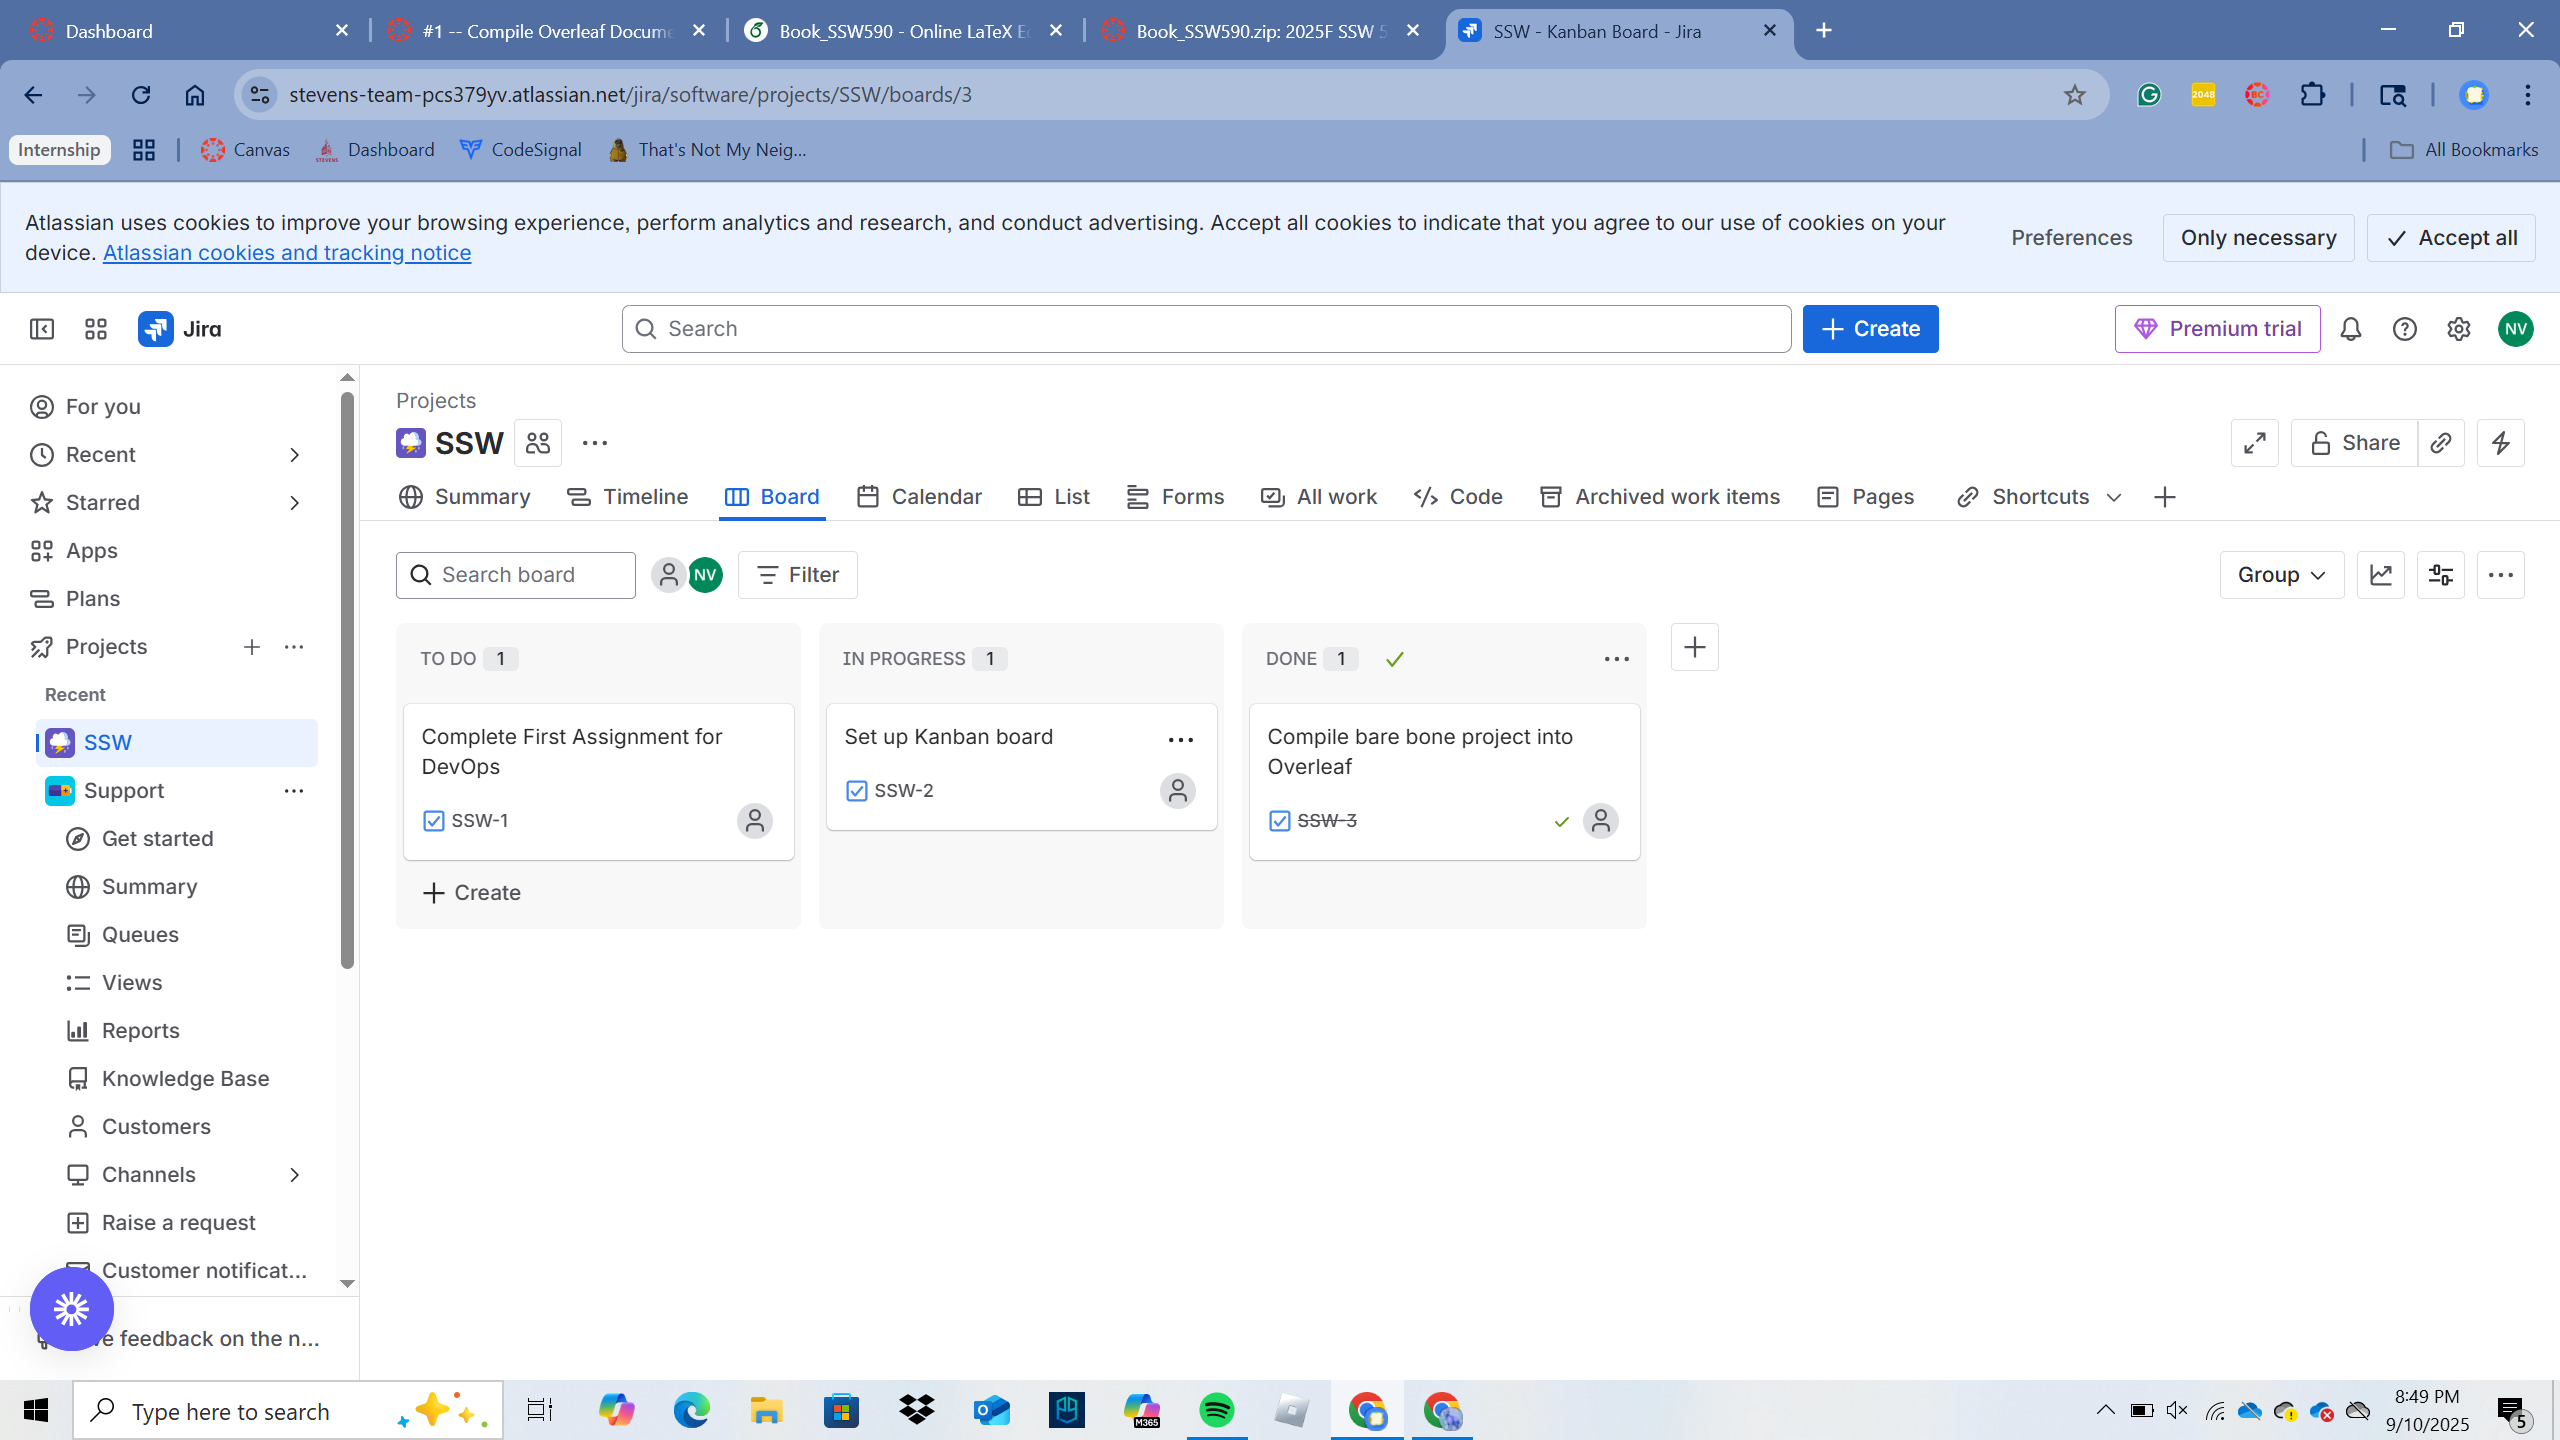
\includegraphics[scale=0.1]{eps/Screenshots/Screenshot (255).png}

\chapter{Passwords \\
\small{\textit{-- Nicole Valdiviezo, Nataly Jimenez, Lakshya Vegiraju}}
\index{Passwords} 
\index{Chapter!Passwords}
\label{Chapter::Passwords}}

The following table defines user accounts, associated servers, and password rules. Actual passwords are not listed; instead, hints are provided to maintain security while offering guidance.

\begin{longtable}{|p{3cm}|p{3cm}|p{3cm}|p{6cm}|}
\caption{Accounts and Password Hints}\label{tab:passwords}\\
\hline
\textbf{User} & \textbf{Server} & \textbf{Rule} & \textbf{Password Hint} \\
\hline
admin & dev-server-1 & Must contain 12+ characters, uppercase, lowercase, number, special character & Based on a twitch streamer manhwa with a year and "!" in between the title.
\hline
developer & dev-server-2 & At least 10 characters, no dictionary words, include numbers & Uses the dog’s name ``Buddy'' combined with reversed birth month digits \\
\hline
tester & staging-server & 8–16 characters, at least 2 special characters & Inspired by ``Five Nights of Freddy's'' character name with two symbols at the start \\
\hline
student (me) & personal-vm & Custom rule: 15+ characters, must include numbers & Name of band from their first concert with the date that they attended \\
root & DigitalOcean droplet(s) & 15+ chars, U/l/d/s & \emph{<key>@do2025!} \\
\hline
admin & Bugzilla (web UI) & 15+ chars, U/l/d/s & \emph{<key>@bugzilla2025!} \\
\hline
admin & Overleaf (web UI) & 15+ chars, U/l/d/s & \emph{<key>@overleaf2025!} \\
\hline
root & DigitalOcean & 12 chars, new droplet as of 10/16 & \emph{aSG252>D.As} \\
\hline

\end{longtable}
\chapter{Hosts \\
\small{\textit{-- Nataly Jimenez, Nicole Valdiviezo, Lakshya Vegiraju}}
\index{Hosts} 
\index{Chapter!Hosts}
\label{Chapter::Hosts}}

The following hosts are defined for the development environment setup:

\begin{longtable}{|p{4cm}|p{6cm}|p{6cm}|}
\caption{Project Hosts}\label{tab:hosts}\\
\hline
\textbf{Host Name} & \textbf{Purpose} & \textbf{Notes} \\
\hline
dev-server-1 & Primary development server & Ubuntu 22.04 VM, used for compiling and running code \\
\hline
dev-server-2 & Backup development server & Red Hat Enterprise Linux, load balancing and redundancy \\
\hline
staging-server & Testing and staging environment & Mirrors production environment, used for pre-deployment tests \\
\hline
db-server & Centralized database host & PostgreSQL instance storing application data \\
do-bugzilla-1 & Bugzilla Docker host & Public: \url{http://165.22.45.163:8081} \\
do-overleaf-1 & Overleaf Docker host & Public: \url{http://165.22.45.163:8080} \\
\hline
\end{longtable}

\chapter{Linux Commands \\
\small{\textit{-- Nataly Jimenez, Nicole Valdiviezo, Lakshya Vegiraju}}
\index{Linux Commands} 
\index{Chapter!Linux Commands}
\label{Chapter::Linux Commands}}

\section{A. Navigation and File Ops}
\subsection{Show your present working directory path only.}
\begin{minted}{bash}
ubuntu@ubuntu:~/lx-test$ pwd
/home/ubuntu/lx-test
\end{minted}

\subsection{List all entries in the current directory, one per line, including dotfiles.}

\begin{minted}{bash}
ubuntu@ubuntu:~/lx-test$ ls -A1
archive
blob.bin
link-to-file1
old.txt
people.csv
src
sys.log
tmp
words.txt
\end{minted}

\subsection{ Copy src/file1.txt to tmp/ only if tmp exists; do it verbosely.}
\begin{minted}{bash}
ubuntu@ubuntu:~/lx-test$ [ -d tmp ] && cp -v src/file1.txt tmp/
'src/file1.txt' -> 'tmp/file1.txt'
\end{minted}

\subsection{ Move old.txt into archive/ and keep its original timestamp.}
\begin{minted}{bash}
ubuntu@nat:~/lx-test$ cp --preserve=timestamps old.txt archive/
ubuntu@nat:~/lx-test$ ls -l old.txt archive/old.txt
-rw-r--r-- 1 ubuntu ubuntu 0 Jan  2  2024 archive/old.txt
-rw-r--r-- 1 ubuntu ubuntu 0 Jan  2  2024 old.txt
\end{minted}

\subsection{ Create a new empty file notes.md only if it does not already exist.}
\begin{minted}{bash}
ubuntu@nat:~/lx-test$ touch -c notes.md
\end{minted}

\subsection{Show disk usage (human-readable) for the src directory only (not total FS).}
\begin{minted}{bash}
ubuntu@ubuntu:~/lx-test$ du -sh src
16K	src
\end{minted}

\section{B. Viewing and Searching}
\subsection{Print line numbers while displaying sys.log.}
\begin{minted}{bash}
ubuntu@nat:~/lx-test$ cat -n sys.log
1  INFO boot ok
2  WARN disk low
3  ERROR fan fail
4  INFO shutdown
\end{minted}

\subsection{Show only the lines in sys.log that contain ERROR (case-sensitive).}
\begin{minted}{bash}
ubuntu@nat:~/lx-test$ grep 'ERROR' sys.log
ERROR fan fail
\end{minted}

\subsection{Count how many distinct words appear in words.txt (case-insensitive).}
\begin{minted}{bash}
ubuntu@nat:~/lx-test$ tr '[:upper:]' '[:lower:]' < words.txt | tr -c '[:alnum:]' '\n' | sort -u | wc -l
3
\end{minted}

\subsection{From words.txt, show lines that start with g or G.}
\begin{minted}{bash}
ubuntu@nat:~/lx-test$ grep -E '^[gG]' words.txt
Gamma
gamma
\end{minted}

\subsection{Display the first 2 lines of people.csv without using an editor.}
\begin{minted}{bash}
ubuntu@nat:~/lx-test$ head -n 2 people.csv
id,name,dept
1,Ada,EE
\end{minted}

\subsection{Show the last 3 lines of sys.log and keep following if the file grows.}
\begin{minted}{bash}
ubuntu@nat:~/lx-test$ tail -n 3 -f sys.log
WARN disk low
ERROR fan fail
INFO shutdown
\end{minted}


\section{C. Text Processing}
\subsection{ From people.csv, print only the name column (2nd), excluding the header.}
\begin{minted}{bash}
ubuntu@nat:~/lx-test$ cut -d',' -f2 people.csv | tail -n +2
Ada
Linus
Grace
\end{minted}

\subsection{ Sort words.txt case-insensitively and remove duplicates.}
\begin{minted}{bash}
ubuntu@nat:~/lx-test$ sort -f words.txt | uniq -i
alpha
beta
Gamma
\end{minted}

\subsection{Replace every three with 3 in all files under src/ in-place, creating .bak backups.}
\begin{minted}{bash}
ubuntu@nat:~/lx-test$ sed -i.bak 's/three/3/g' src/*.txt
ubuntu@nat:~/lx-test$ ls src/*.bak
src/file1.txt.bak  src/file2.txt.bak
\end{minted}

\subsection{ Print the number of lines, words, and bytes for every *.txt file in src/.}
\begin{minted}{bash}
ubuntu@nat:~/lx-test$ wc src/*.txt
 1  4 15 src/file1.txt
 1  4 16 src/file2.txt
 2  8 31 total
\end{minted}

\section{D. Permissions and Ownership}
\subsection{Make tmp/ readable, writable, and searchable only by the owner.}
\begin{minted}{bash}
$ chmod 700 tmp
$ ls -ld tmp
drwx------ 2 username username 4096 Sep 16 09:00 tmp

\end{minted}

\subsection{ Give group execute permission to src/lib recursively without touching others/owner bits.}
\begin{minted}{bash}
$ chmod -R g+x src/lib

\end{minted}

\subsection{ Show the numeric (octal) permissions of src/file2.txt.}
\begin{minted}{bash}
$ stat -c "%a %n" src/file2.txt
644 src/file2.text
\end{minted}

\subsection{ Make notes.md append-only for the owner via file attributes (if supported)}
\begin{minted}{bash}
$ chattr +a notes.md
$ lsattr notes.md
-----a--------e----notes.md
\end{minted}

\section{ E) Links and Find}
\subsection{Verify whether link-to-file1 is a symlink and show its target path.}
\begin{minted}{bash}
$ ls -l link-to-file1
lrwxrwxrwx 1 username username 12 Sep 16 09:00 link-to-file1 ->src/file1.txt
\end{minted}

\subsection{Find all regular files under the current tree larger than 40 KiB.}
\begin{minted}{bash}
$ find . -type f -size +40k
./blob.bin
\end{minted}

\subsection{Find files modified in the last 10 minutes under tmp/ and print their sizes.}
\begin{minted}{bash}
$ find tmp/ -type f -mmin -10 -exec ls -lh {} \;
-rw-r--r-- 1 username username 24 Sep 16 10:10 tmp/file1.txt
-rw-r--r-- 1 username username 24 Sep 16 10:11 tmp/file2.txt
\end{minted}

\section{F) Processes and Job Control}
\subsection{Show your processes in a tree view.}
\begin{minted}{bash}
$ pstree -u username
systemd───gnome-terminal───bash───pstree
\end{minted}

\subsection{Start sleep 120 in the background and show its PID.}
\begin{minted}{bash}
$ sleep 120 &
[1] 24567
\end{minted}

\subsection{Send a TERM signal to all sleep processes owned by you (don’t use kill -9).}
\begin{minted}{bash}
$ pkill -TERM -u $USER sleep
\end{minted}

\subsection{Show the top 5 processes by memory usage (one-shot, not interactive).}
\begin{minted}{bash}
$ ps -eo pid,comm,%mem --sort=-%mem | head -n 6
  PID COMMAND     %MEM
 1324 firefox     12.0
 1401 gnome-shell  8.5
 1256 code         7.3
 2456 bash         1.0
 2457 ps           0.5
\end{minted}

\section{ G) Archiving and Compression}
\subsection{Create a gzipped tar archive src.tgz from src/ with relative paths.}
\begin{minted}{bash}
$ tar -czf src.tgz src
\end{minted}

\subsection{List the contents of src.tgz without extracting.}
\begin{minted}{bash}
$ tar -tzf src.tgz
src/
src/file1.txt
src/file2.txt
src/lib/
\end{minted}

\subsection{Extract only file2.txt from src.tgz into tmp/.}
\begin{minted}{bash}
$ tar -xzf src.tgz -C tmp src/file2.txt
\end{minted}

\section{ H) Networking and System Info}
\subsection{Show all listening TCP sockets with associated PIDs (no root assumptions).}
\begin{minted}{bash}
ss -ltpn
\end{minted}

\subsection{Print your default route (gateway) in a concise form.}
\begin{minted}{bash}
ip route | grep '^default'
\end{minted}

\subsection{Display kernel name, release, and machine architecture.}
\begin{minted}{bash}
uname -srm
\end{minted}

\subsection{ Show the last 5 successful logins (or last sessions) on the system.}
\begin{minted}{bash}
last -n 5
\end{minted}

\section{ I) Package and Services (Debian/Ubuntu)}
\subsection{Show the installed version of package coreutils.}
\begin{minted}{bash}
dpkg -s coreutils | grep '^Version:'
\end{minted}

\subsection{Search available packages whose names contain ripgrep.}
\begin{minted}{bash}
apt-cache search ripgrep
\end{minted}

\subsection{Check whether service cron is active and print its status line only.}
\begin{minted}{bash}
systemctl status cron | grep 'Active:'
\end{minted}

\section{ J) Bash and Scripting}
\subsection{Write a one-liner that loops over *.txt in src/ and prints: : .}
\begin{minted}{bash}
for f in src/*.txt; do echo "$f : $(wc -l < "$f")"; done
\end{minted}

\subsection{Write a command that exports CSV rows where dept == "CS" to cs.txt (exclude header).}
\begin{minted}{bash}
awk -F, 'NR>1 && $2=="CS"' people.csv > cs.txt
\end{minted}

\subsection{Create a variable X with value 42, print it, then remove it from the environment}
\begin{minted}{bash}
export X=42; echo $X; unset X
\end{minted}
\chapter{Project Proposal \\
\small{\textit{-- Nataly Jimenez, Nicole Valdiviezo, Lakshya Vegiraju}}
\index{Project Proposal} 
\index{Chapter!Project Proposal}
\label{Chapter::Project Proposal}}

\section*{Project Title}
HTML Drawings Dance to Music

\section*{Project Description}
The goal of this project is to create a dynamic web-based application that combines audio and visual elements using vanilla JavaScript and the HTML5 Canvas element. The application will allow shapes and colors to move and transform in response to music, ultimately producing beautiful audio visualizations.  

A sample task includes building an interactive music visualizer that reacts in real time to user-selected audio files. The project will start from the basics of drawing shapes on a canvas and gradually progress to more advanced features such as frequency analysis, animation techniques, and synchronization with audio events.  

The project will also explore integrating DevSecOps tools to manage the lifecycle, ensuring secure, maintainable, and automated development practices.  

\subsection*{Potential DevSecOps Tools}
\begin{itemize}
    \item \textbf{Source Control:} GitHub for version control and collaborative development.
    \item \textbf{Testing:} Jest (JavaScript testing framework) to validate audio analysis and canvas rendering functions.
    \item \textbf{Deployment:} GitHub Pages or AWS Amplify for hosting the web application.
    \item \textbf{Databases:} (Optional) Firebase or AWS DynamoDB for saving user preferences, visualizer settings, or playlists.
    \item \textbf{CI/CD Pipelines:} GitHub Actions for automated builds, testing, and deployments.
    \item \textbf{Monitoring:} AWS CloudWatch or open-source tools like Grafana/Prometheus for operational monitoring.
    \item \textbf{Security:} Dependabot (via GitHub) for vulnerability scanning, ESLint for secure code checks.
\end{itemize}

\section*{Expectations / Rubric}
The project will be evaluated based on the following criteria:

\begin{enumerate}
    \item \textbf{Selected Tool(s) or Environment} 
    \item \textbf{Building a Sample Working Application (40 pts)}  
    Development of an HTML5 Canvas audio visualizer application.
    
    \item \textbf{Using Specific Tools (DevOps tools) (20 pts)}  
    Integration of version control (GitHub), testing (Jest), deployment (AWS Amplify vs GitHub Pages), and monitoring tools. A comparison will be made between two hosting solutions.
    
    \item \textbf{Environment to Build the Project (20 pts)}  
    Hosting on AWS Amplify and GitHub Pages, with automated pipelines (GitHub Actions).
    
    \item \textbf{Operational Dashboard (20 pts)}  
    A monitoring dashboard (Grafana or CloudWatch) to reflect performance and operational aspects of the web app.
    
    \item \textbf{SWOT Chart (20 pts)}  
    A customized SWOT analysis for each major tool (e.g., GitHub Pages vs AWS Amplify).
    
    \item \textbf{Propose Something Unique}  
    Demonstrating real-time visualization of custom audio input (user-uploaded MP3 or live microphone input) for creative coding projects.
\end{enumerate}

\chapter{AWS Deployment \\
\small{\textit{-- Nataly Jimenez, Nicole Valdiviezo, Lakshya Vegiraju}}
\index{AWS Deployment} 
\index{Chapter!AWS Deployment}
\label{Chapter::AWS Deployment}}

This chapter documents step-by-step how to deploy the Two Buttons website to AWS using ECR + App Runner. The color buttons application was successfully deployed to Amazon Web Services using ECR and ECS with Fargate.

\section{Verifying If AWS CLI Is Already Installed}

\begin{minted}{bash}
aws --version
# Returned: 
\end{minted}

\section{Post-Install Configuration and Confirming Credentials Are Working}
\begin{minted}{bash}
aws configure sso:
# Example answers:
# SSO session name: my-sso
# SSO start URL: https://YOUR-SUBDOMAIN.awsapps.com/start
# SSO region: us-east-2
# Account: <select>
# Role:
AdministratorAccess (or your role)
# Default region: us-east-2
# Output: json
# Login
aws sso login --profile default
aws configure# AWS Access Key ID: <AKIA...>
# AWS Secret Access Key: <...>
# Default region name: us-east-2
# Default output format: json
ws sts get-caller-identity
\end{minted}

\section{Create AWS Account}
1. Go to aws.amazon.com → Create an AWS Account.
2. Log in as the root user once to complete setup.
3. Enable MFA on the root account: AWS Console → IAM → Dashboard → Activate MFA on
your root account. Store recovery codes safely.
4. Choose a home region (e.g., us-east-2) and use it consistently in commands

\section{Set Cost Budget}
1. Console: Billing → Budgets → Create budget.
2. Budget type: Cost budget, amount e.g. \$10/month.
3. Configure alerts at 50\%, 80\%, and 100\% to your email.

\section{Enable IAM Identity Center (SSO)}
1. Console: IAM Identity Center → Enable.
2. Create a user for yourself (e.g., your work email)
3. Create or assign a Permission Set: start with AdministratorAccess. (You can later add a
least-privilege set for ECR push.)
4. Record your SSO Start URL (you’ll need it in the CLI).

\section{Install and Configure AWS CLI for SSO}

\begin{minted}{bash}
sudo apt-get update && sudo apt-get install -y unzip
curl "https://awscli.amazonaws.com/awscli-exe-linux-x86_64.zip" -o "awscliv2.zip"
unzip awscliv2.zip && sudo ./aws/install
aws configure sso# Prompts (example answers):
# SSO session name: my-sso
# SSO start URL: https://YOUR-SUBDOMAIN.awsapps.com/start
# SSO region: us-east-2
# Account: <select your new account>
# Role: AdministratorAccess
# Default region: us-east-2
# Output: json
# Log in via browser:
aws sso login --profile default
\end{minted}

\section{Set Environmental Variables}
\begin{minted}{bash}
# >>> EDIT THESE <<<
export AWS_REGION=us-east-1
export ECR_REPO=myapp
export IMAGE_TAG=v1
export CONTAINER_PORT=3000
# Port your app listens on
# Discover your AWS Account ID from your SSO session:
export AWS_ACCOUNT_ID="$(aws sts get-caller-identity --query Account --output text --profile default)"
\end{minted}

\section{Create an ECR Repo}
\begin{minted}{bash}
aws ecr describe-repositories \
--repository-names "$ECR_REPO" \
--region "$AWS_REGION" --profile default >/dev/null 2>&1 || \
aws ecr create-repository \
--repository-name "$ECR_REPO" \
--image-scanning-configuration scanOnPush=true \
--region "$AWS_REGION" --profile default
\end{minted}

\section{Authenticate Docker to ECR}
\begin{minted}{bash}
aws ecr get-login-password --region "$AWS_REGION" --profile default \
| docker login --username AWS --password-stdin \
"$AWS_ACCOUNT_ID.dkr.ecr.$AWS_REGION.amazonaws.com"
\end{minted}

\section{Build, Tag and Push Local Image}
\begin{minted}{bash}
docker build --platform linux/amd64 -t "$ECR_REPO:$IMAGE_TAG" .
# Tag it for ECR
docker tag "$ECR_REPO:$IMAGE_TAG" \
"$AWS_ACCOUNT_ID.dkr.ecr.$AWS_REGION.amazonaws.com/$ECR_REPO:$IMAGE_TAG"
# Push to ECR
docker push "$AWS_ACCOUNT_ID.dkr.ecr.$AWS_REGION.amazonaws.com/$ECR_REPO:$IMAGE_TAG"
\end{minted}

\section{Verify Image in ECR}
\begin{minted}{bash}
aws ecr describe-images \
--repository-name "$ECR_REPO" \
--region "$AWS_REGION" --profile default \
--query 'imageDetails[].imageTags'
\end{minted}


\section{Quick Deploy with App Runner}
\begin{minted}{bash}
export APP_NAME=my-apprunner-app
aws apprunner create-service \
--service-name "$APP_NAME" \
--region "$AWS_REGION" --profile default \
--source-configuration "{
\"ImageRepository\": {
\"ImageIdentifier\": \"$AWS_ACCOUNT_ID.dkr.ecr.$AWS_REGION.amazonaws.com/$ECR_REPO:$IMAGE_TAG\",
\"ImageRepositoryType\": \"ECR\",
\"ImageConfiguration\": {\"Port\": \"$CONTAINER_PORT\"}
},
\"AutoDeploymentsEnabled\": true
}" \
--instance-configuration "{\"Cpu\":\"1 vCPU\",\"Memory\":\"2 GB\"}"

AWS_REGION=us-east-2
PROFILE=AdministratorAccess-539272219501
SERVICE_ARN=arn:aws:apprunner:us-east-2:539272219501:service/my-apprunner-app/04c50b98cd0744369e395b654752a33c

while true; do
STATUS=$(aws apprunner describe-service \
--service-arn "$SERVICE_ARN" \
--region "$AWS_REGION" --profile "$PROFILE" \
--query 'Service.Status' --output text)
echo "Service status: $STATUS"
case "$STATUS" in RUNNING|CREATE_FAILED|OPERATION_FAILED) break ;; esac
sleep 4
done

aws apprunner list-services \
--region "$AWS_REGION" --profile default \
--query "ServiceSummaryList[?ServiceName=='$APP_NAME'].ServiceUrl" --output text
\end{minted}

\section{Security Checklist}
MFA enabled on the root account and your SSO user. Used SSO (no long-lived access keys on laptops). Cost budget with email alerts. Principle of least privilege for day-2 (created a minimal ECR Push permission set)

\section{AWS Website}
Links to AWS Website: 
\begin{verbatim}
    http://18.224.136.57:3000
\end{verbatim}
This is a dynamic public IP address assigned by AWS Fargate. The IP address will change if the task is stopped and restarted.

\section{AWS Account and Region Information}
\begin{itemize}
    \item UserId: AIDAZVOAA2MH4K2XESOC4
    \item AWS Acount ID: 664512025359
    \item Access Key: ****************ZGVP
    \item Region: us-east-2 (US East - Ohio)
    \item IAM User: ncvald
\end{itemize}

\section{ECS Deployment Information}

\begin{itemize}
    \item Cluster Name: my-cluster1
    \item Task Definition: color-buttons-task
    \item Service Type: AWS Fargate
    \item Container Port: 3000
\end{itemize}
\section{ECR Repository Information}
\begin{itemize}
    \item ECR Repository Name: color-button-app
    \item ECR Repository URI: 664512025359.dkr.ecr.us-east-2.amazonaws.com/color-button-app
    \item Image Tags: v1 (original), v2 (class-based JavaScript)
\end{itemize}

\section{Deployment Versions}
\begin{itemize}
    \item Version 1 (v1): Original implementation with function-based JavaScript.
    \\ Image URI: 664512025359.dkr.ecr.us-east-2.amazonaws.com/color-button-app:v1
    \item Version 2 (v2): Updated implementation with class-based JavaScript (current)
    \\Image URI: 664512025359.dkr.ecr.us-east-2.amazonaws.com/color-button-app:v2
    
\end{itemize}

\section{Images}

Below are images showing the color button app, the ECS task showing a RUNNING status, and the task details page showing the public IP
\begin{figure}
    \centering
    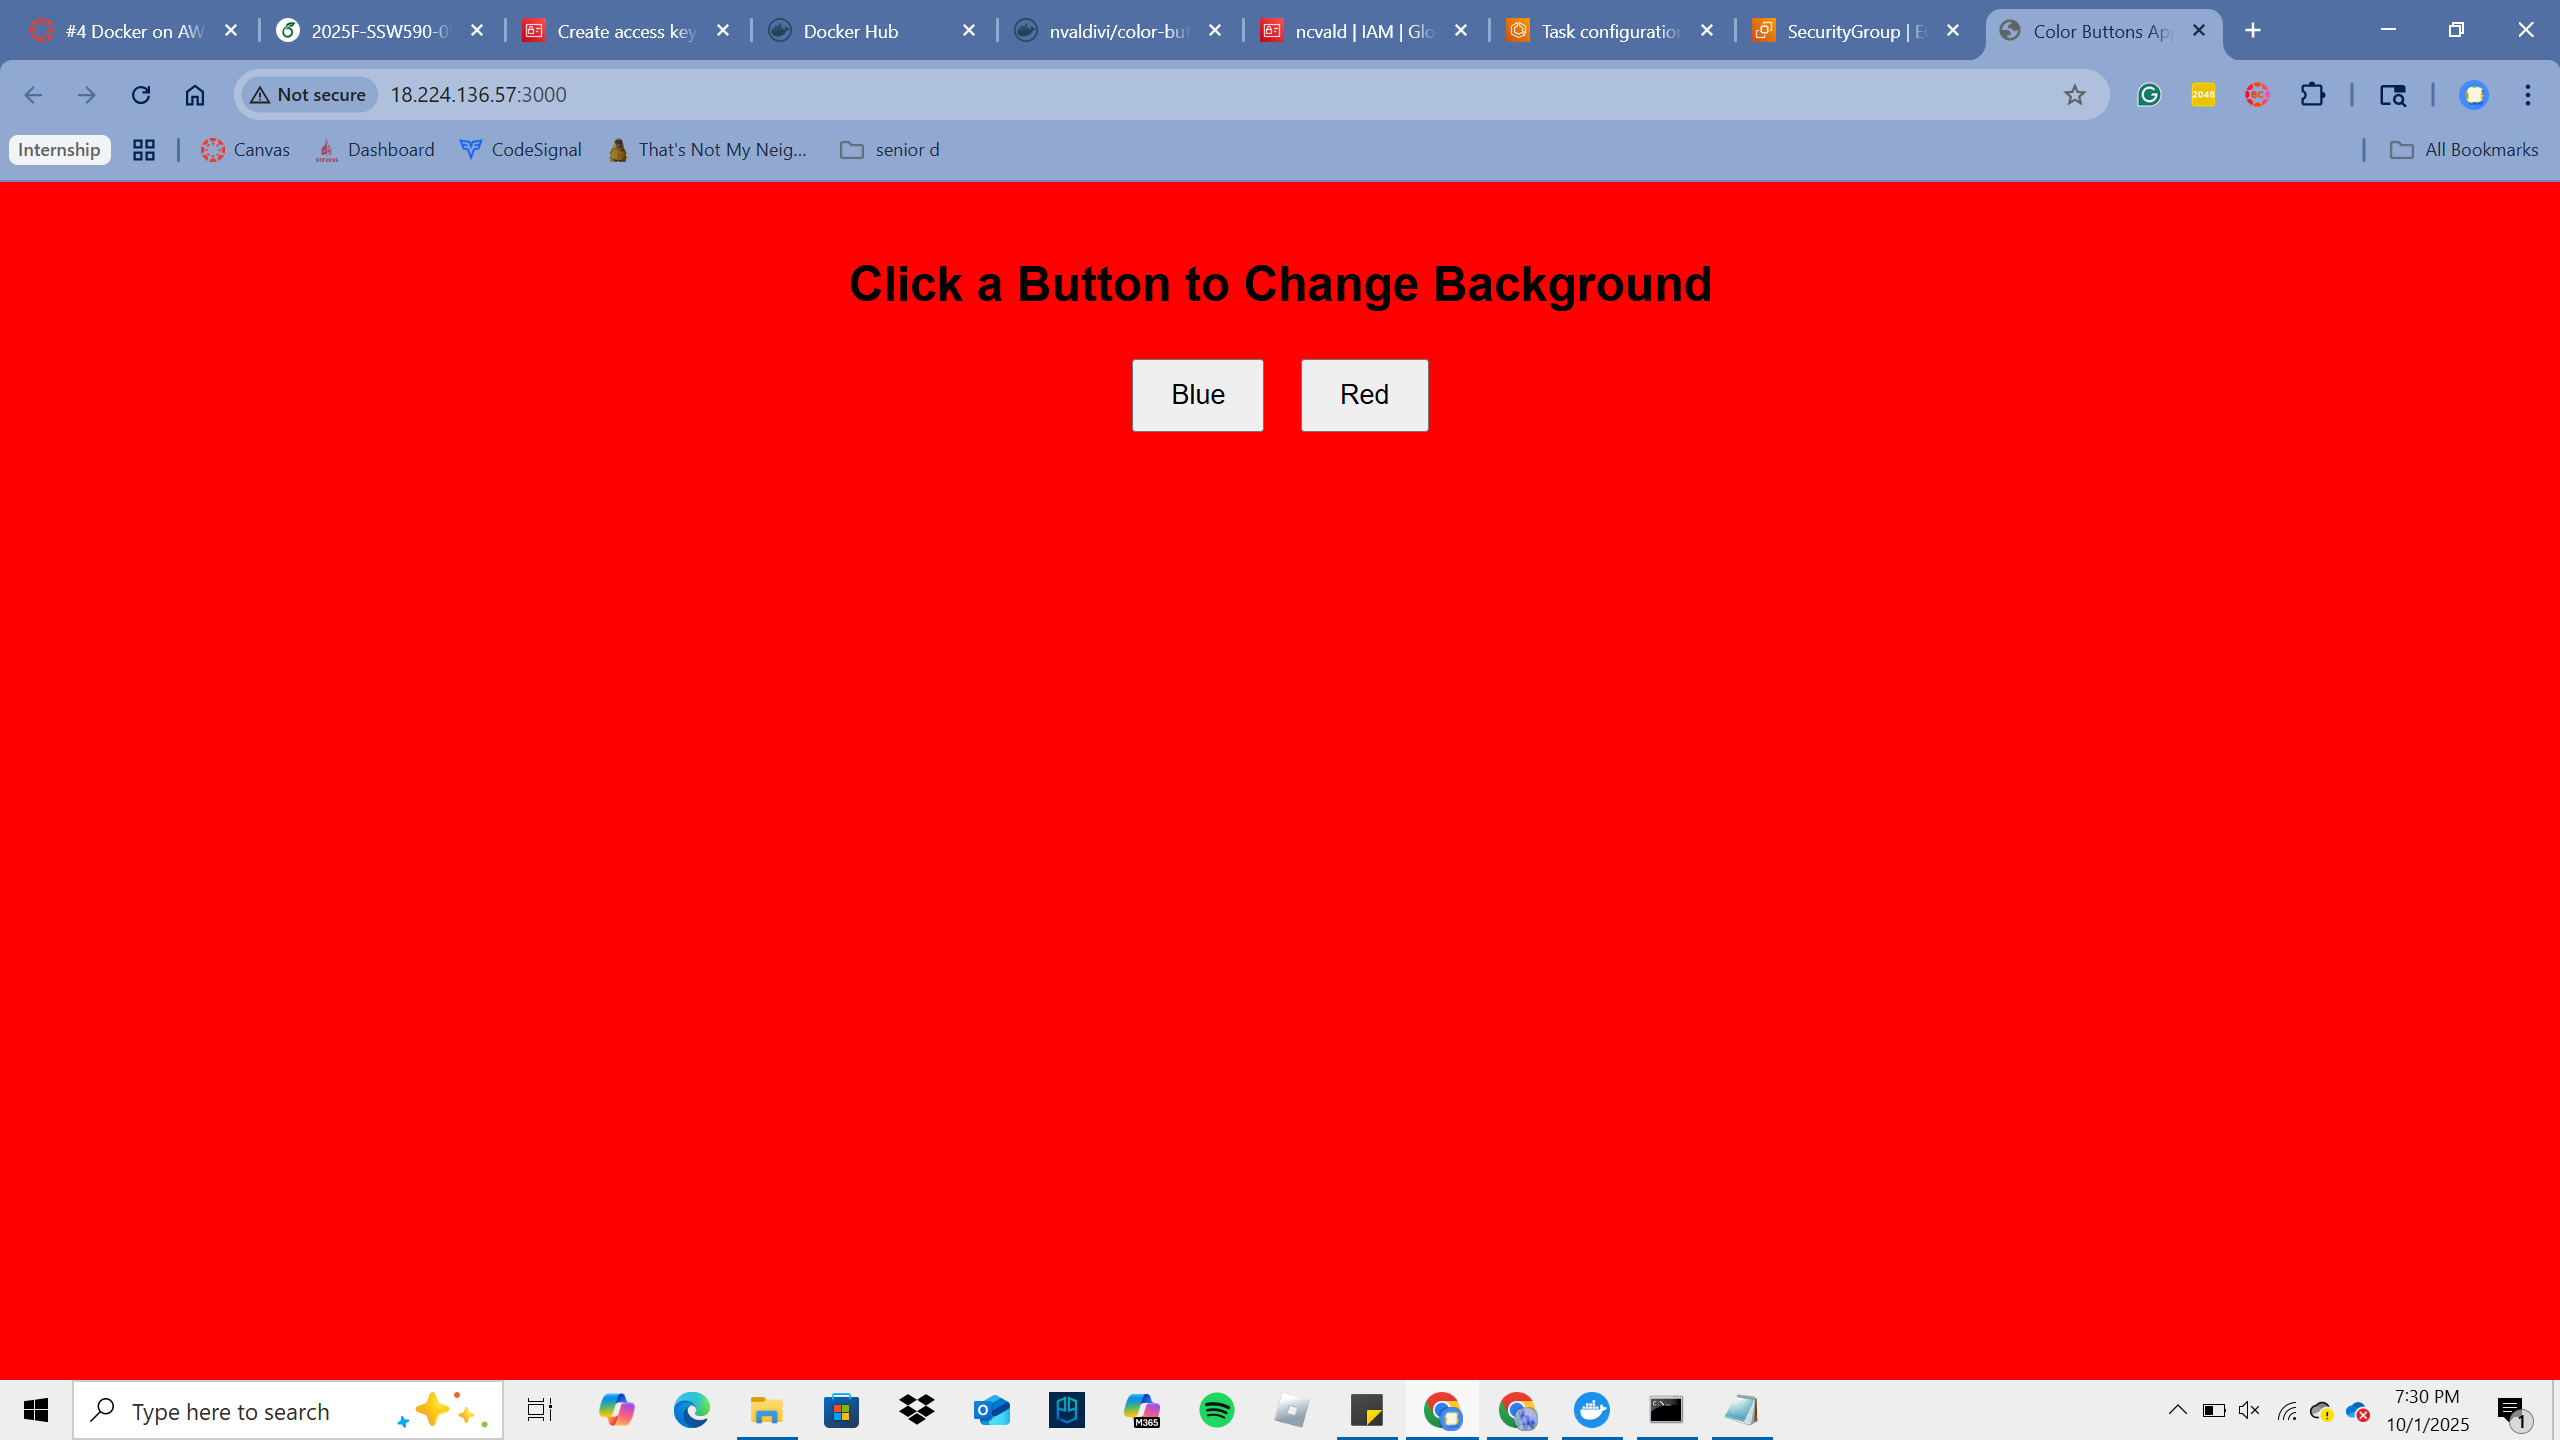
\includegraphics[width=0.6\linewidth]{Book_SSW590 (1)/eps/Screenshots/NewColorButton.png}
    \caption{Color Buttom App V2}
    \label{fig:Color Buttom App V2}
\end{figure}

\begin{figure}
    \centering
    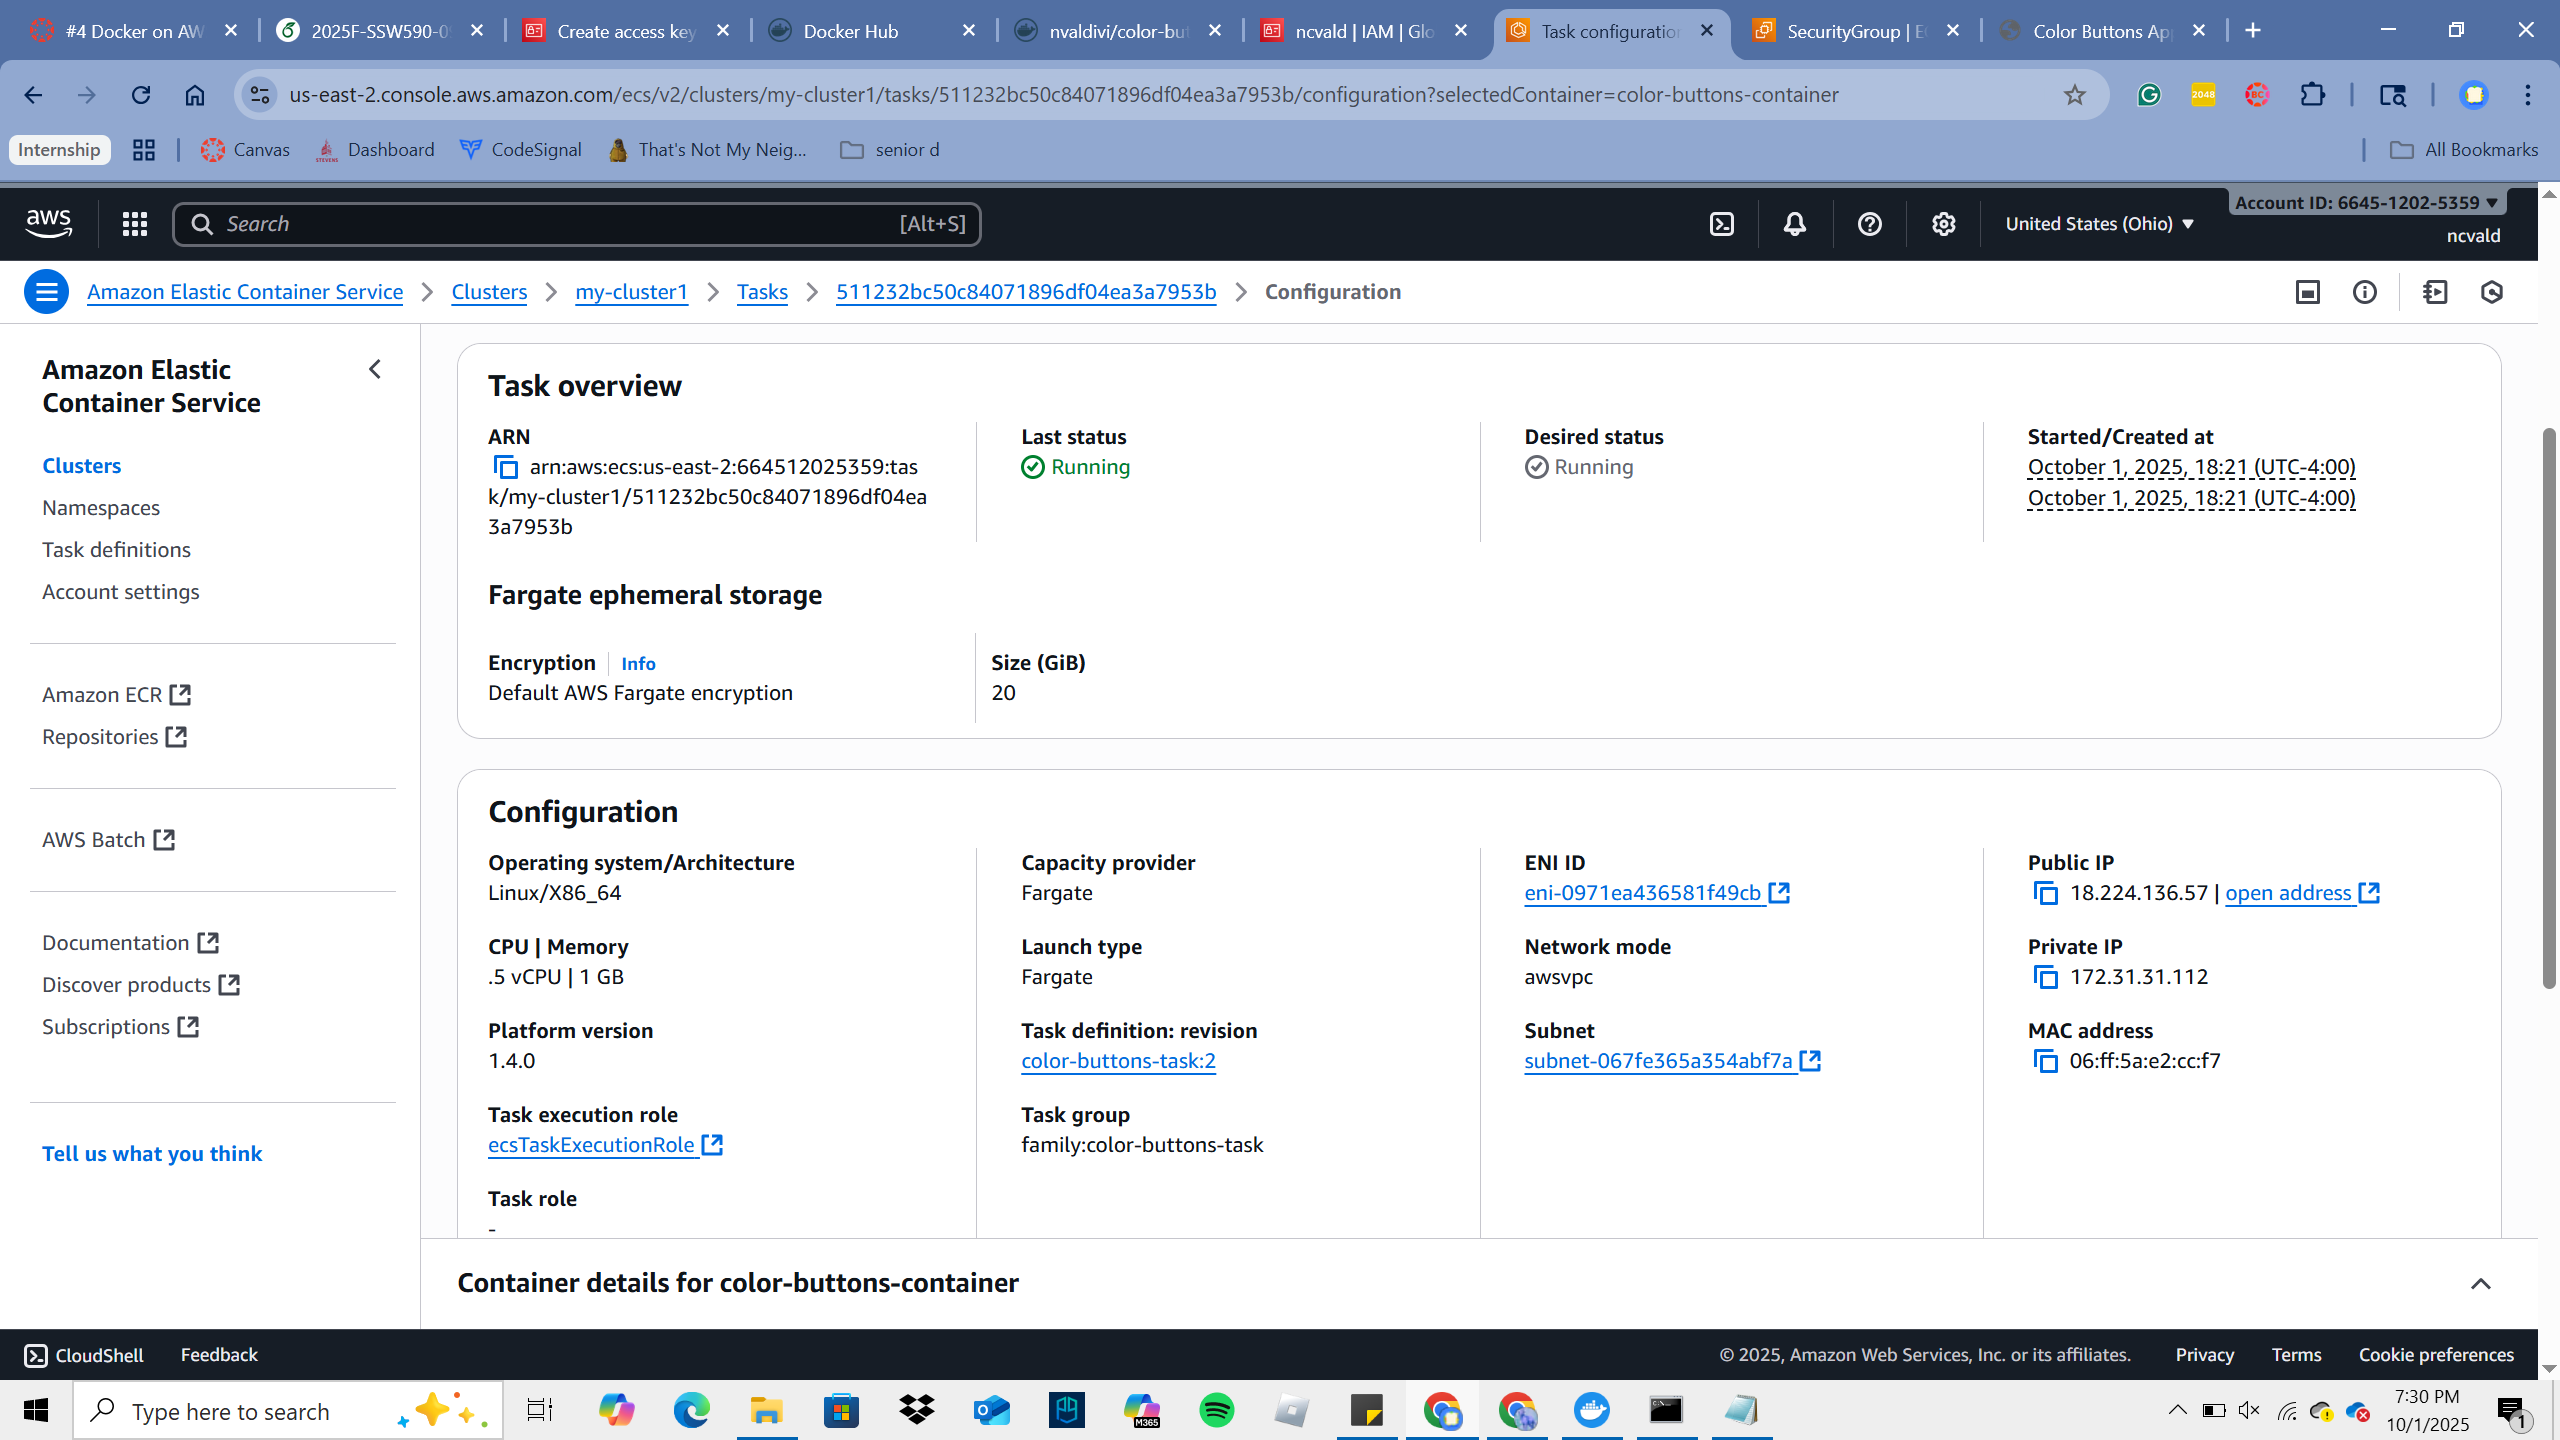
\includegraphics[width=0.6\linewidth]{Book_SSW590 (1)/eps/Screenshots/PublicIP.png}
    \caption{Public IP}
    \label{fig:Public IP}
\end{figure}

\begin{figure}
    \centering
    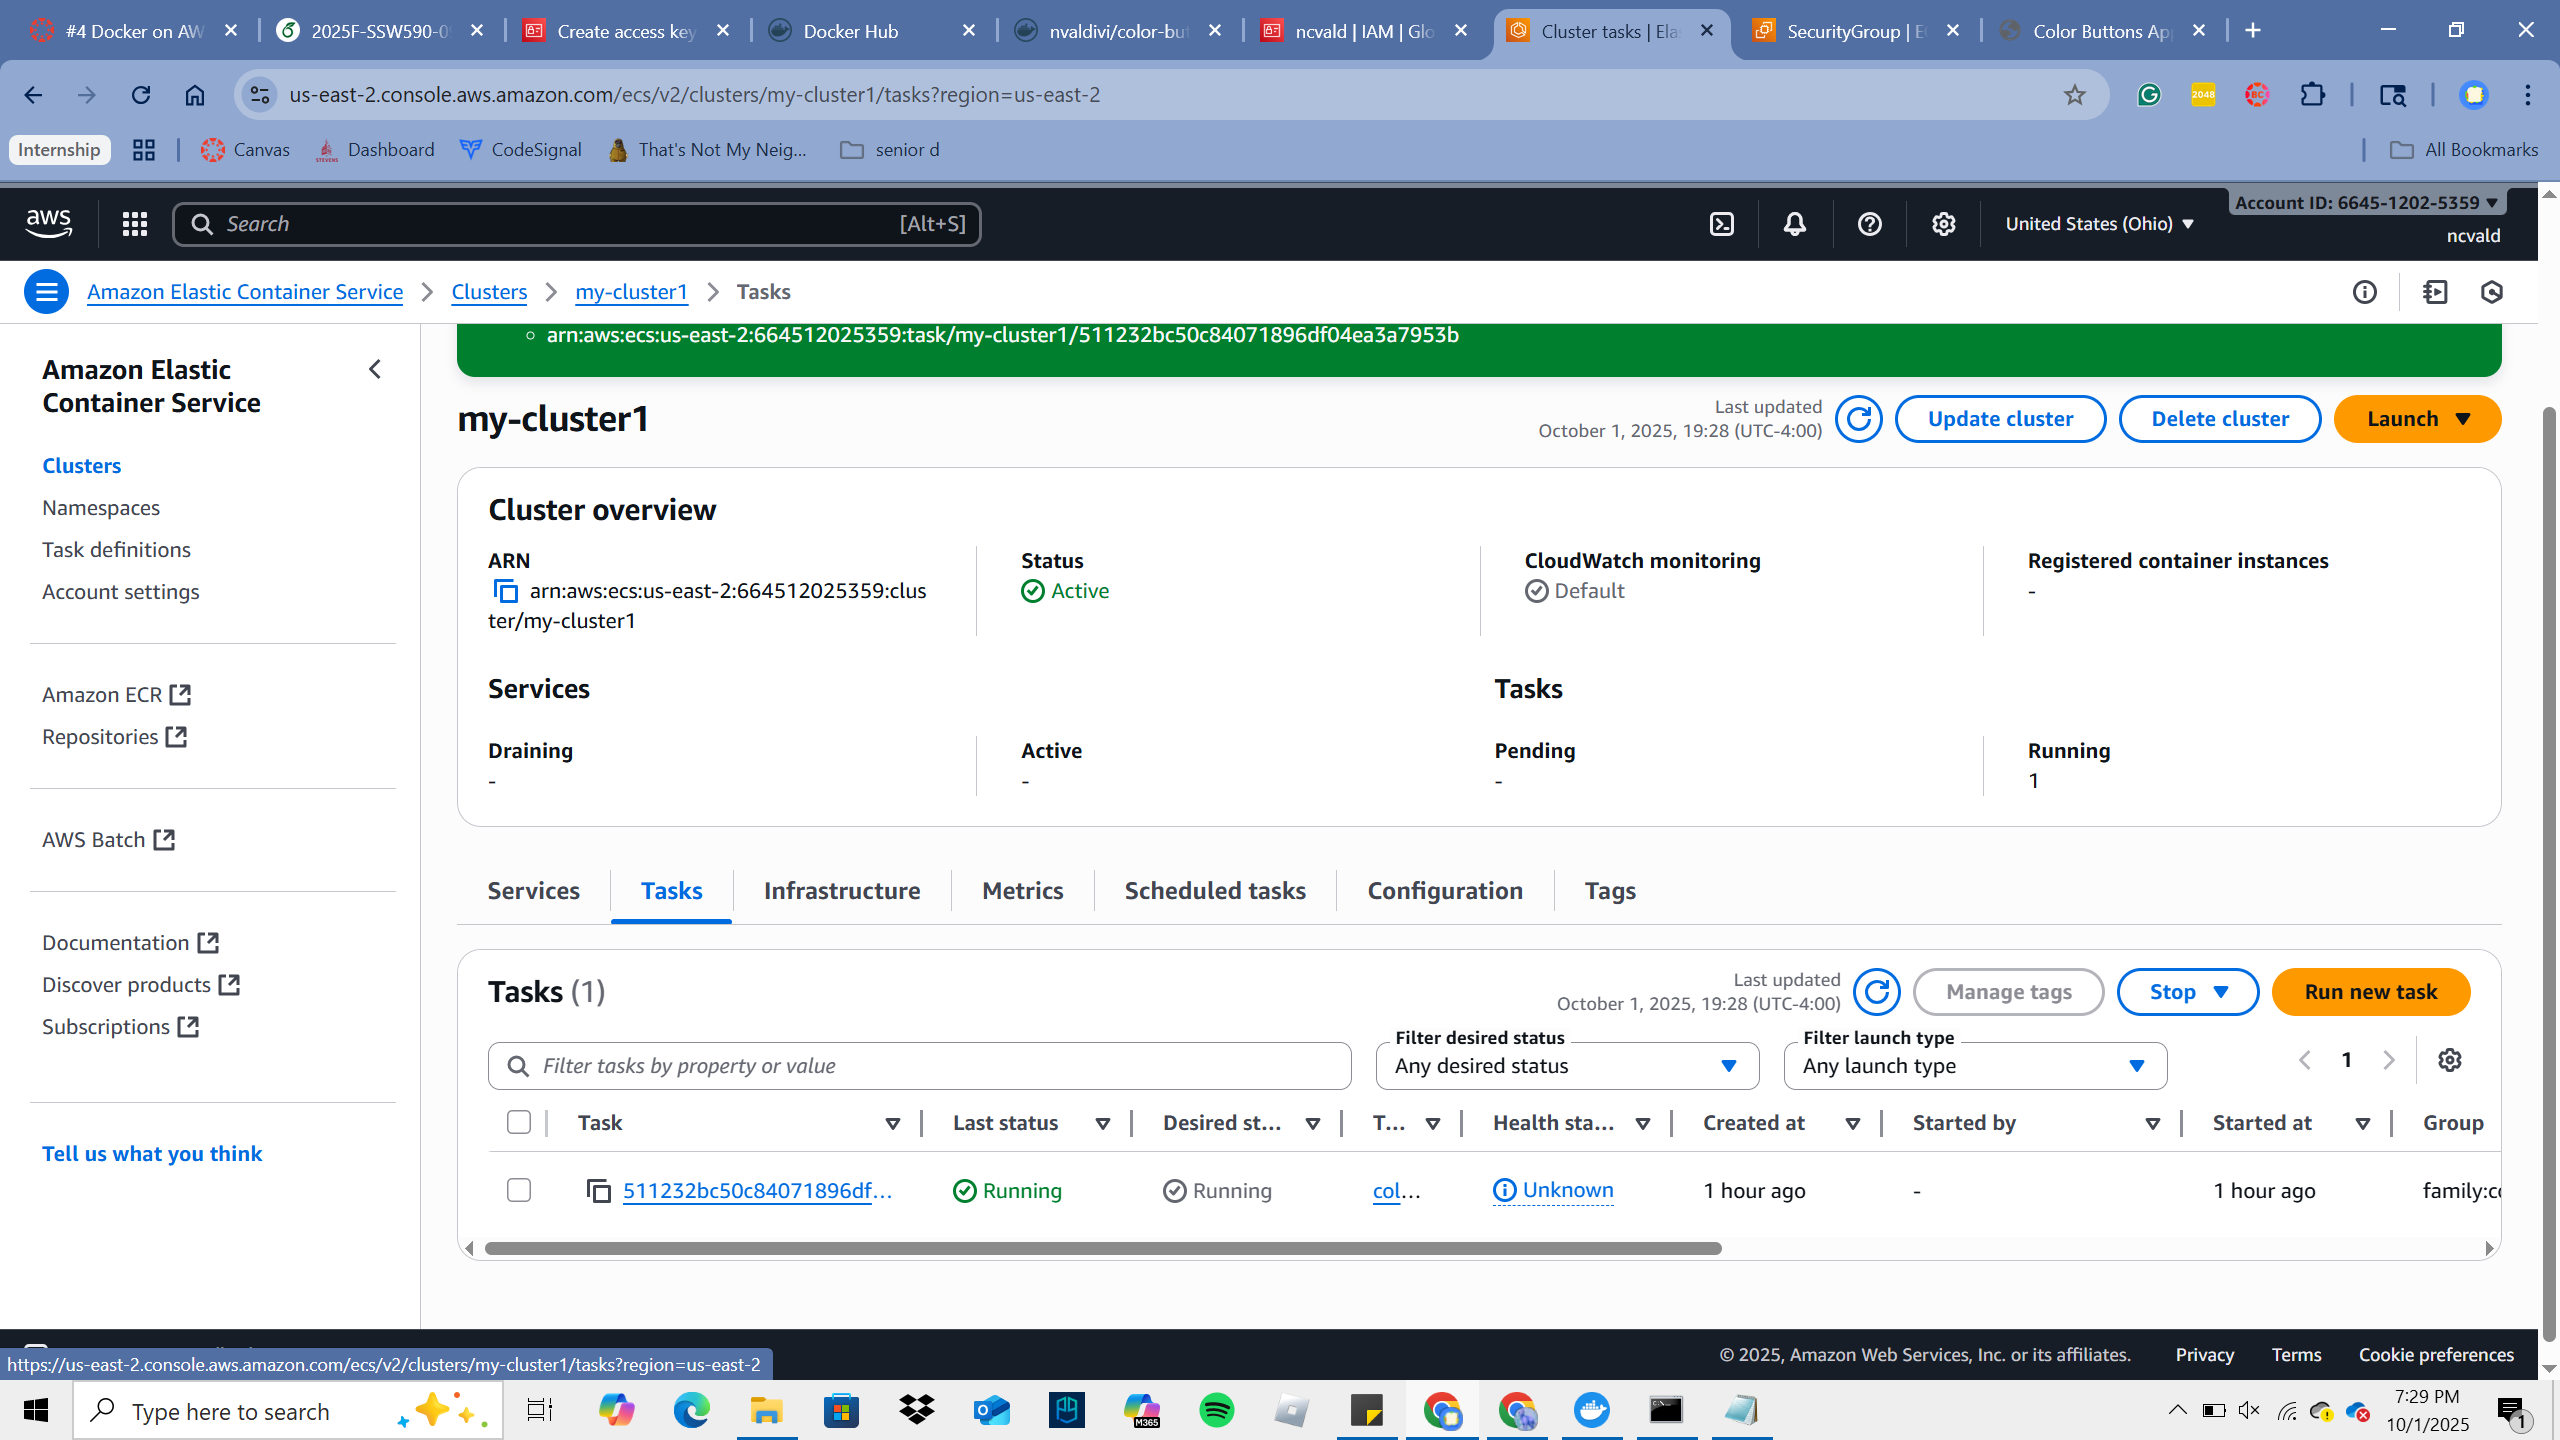
\includegraphics[width=0.6\linewidth]{Book_SSW590 (1)/eps/Screenshots/TaskRunning.png}
    \caption{Task Running}
    \label{fig:Tasking Running}
\end{figure}

\section{UML Class Design}
Below is an image of the UML class diagram for the updated design: changing the website for the two buttons to use a class-based javascript instead of methods: 

\begin{figure}[htbp]
\centering
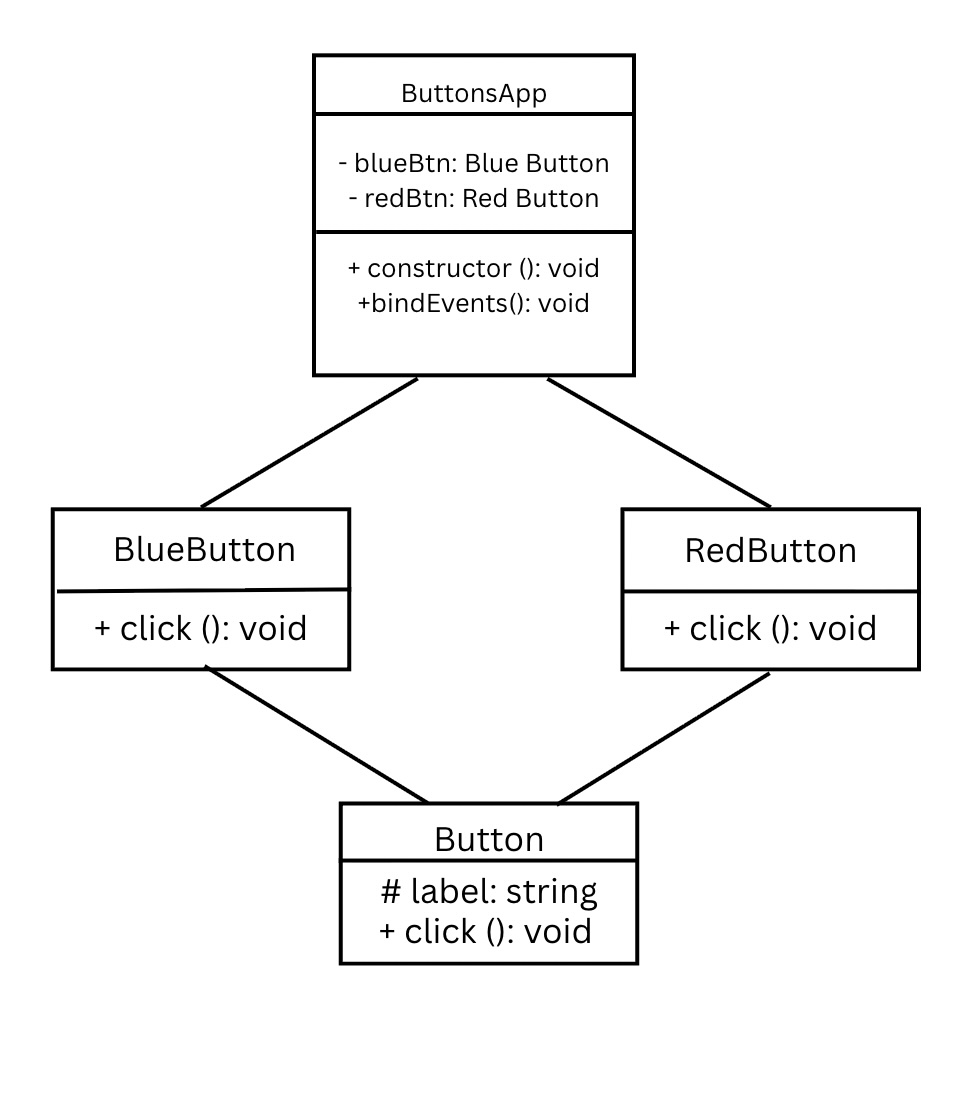
\includegraphics[width=0.85\linewidth]{uml_diagram.jpg}
\caption{UML class diagram for the class-based two-buttons app}
\label{fig:uml-diagram}
\end{figure}
\chapter{LaTeX Docker \\
\small{\textit{-- Nataly Jimenez, Nicole Valdiviezo, Lakshya Vegiraju}}
\index{LaTeX Docker} 
\index{Chapter!LaTeX Docker}
\label{Chapter::LaTeX Docker}}

In this chapter, we demonstrate how to use Docker to compile a simple 
\LaTeX{} document. This approach mirrors the toolchain used by Overleaf, 
which relies on \text{TeX Live}. By containerizing \LaTeX{} compilation, 
we ensure reproducibility and portability across systems.

\section{Dockerfile}
We start by writing a \text{Dockerfile} that installs \text{TeX Live} 
inside a minimal Linux container.

\begin{minted}{Docker}
FROM texlive/texlive:latest

# Install any additional packages if needed
RUN apt-get update && apt-get install -y \
    make \
    latexmk \
    python3-pygments && \
    rm -rf /var/lib/apt/lists/*

# Set working directory
WORKDIR /data

# Default command: compile LaTeX using latexmk
CMD ["latexmk", "-pdf", "main.tex"]
\end{minted}

\section{Sample LaTeX Document}
We will compile a very simple LaTeX file, named \texttt{main.tex}. This file 
serves as a proof-of-concept.

\texttt{\textbackslash section\{Hello, Docker!\}}

This is a minimal LaTeX document compiled inside a Docker container.

\section{Building and Running the Container}
To build and run the Docker container, use the following commands:

\begin{minted}{bash}
# Build the Docker image
docker build -t latex-docker .

# Run the container with a mounted volume
docker run --rm -v $(pwd):/data latex-docker
\end{minted}

After running the above commands, you should see \text{main.pdf} generated 
in your working directory. This workflow mirrors Overleaf’s approach to 
LaTeX document compilation using TeX Live in a controlled environment.
\chapter{Bugzilla \\
\small{\textit{-- Nataly Jimenez, Nicole Valdiviezo, Lakshya Vegiraju}}
\index{Bugzilla} 
\index{Chapter!Bugzilla}
\label{Chapter::Bugzilla}}


\section{Overview}
Bugzilla is an open-source bug tracking system used by software development teams to manage software defects. The team deployed Bugzilla as a Docker container on a DigitalOcean Droplet using GitHub Student Developer Pack credits. Containerization simplifies deployment, ensures consistency, and allows easy management alongside other tools like Overleaf.

\section{Configuration Steps}

\subsection{Setup Bugzilla Docker Container}
Step 1. Create a Droplet through https://cloud.digitalocean.com/droplets

Click Create Droplet
Under Choose an image, select:
Docker (Marketplace tab) → Click Docker on Ubuntu
Choose:
Basic plan (the cheapest, \$6/month)

Region:  NYC3

Authentication: choose Password (make a strong one)

Click Create Droplet
Once it's running:
Public IP address: 165.22.45.163

\subsection{Connect via SSH}
\begin{minted}{bash}
ssh root@165.22.45.163
\end{minted}

\subsection{Run Bugzilla in Docker}
To set up Bugzilla, I deployed a Docker container on DigitalOcean using the official Apache HTTP image (httpd) as a base web environment to simulate Bugzilla deployment (since public Bugzilla images are deprecated).

After creating the Droplet (Docker on Ubuntu), I connected via SSH and ran:
\begin{minted}{bash}
docker run -d -p 8081:80 --name bugzilla httpd
http://165.22.45.163:8081
\end{minted}

\section{Images}
The following screenshots provide evidence of assignment completion for the Bugzilla section of the project:


\begin{figure}[ht]
    \centering
    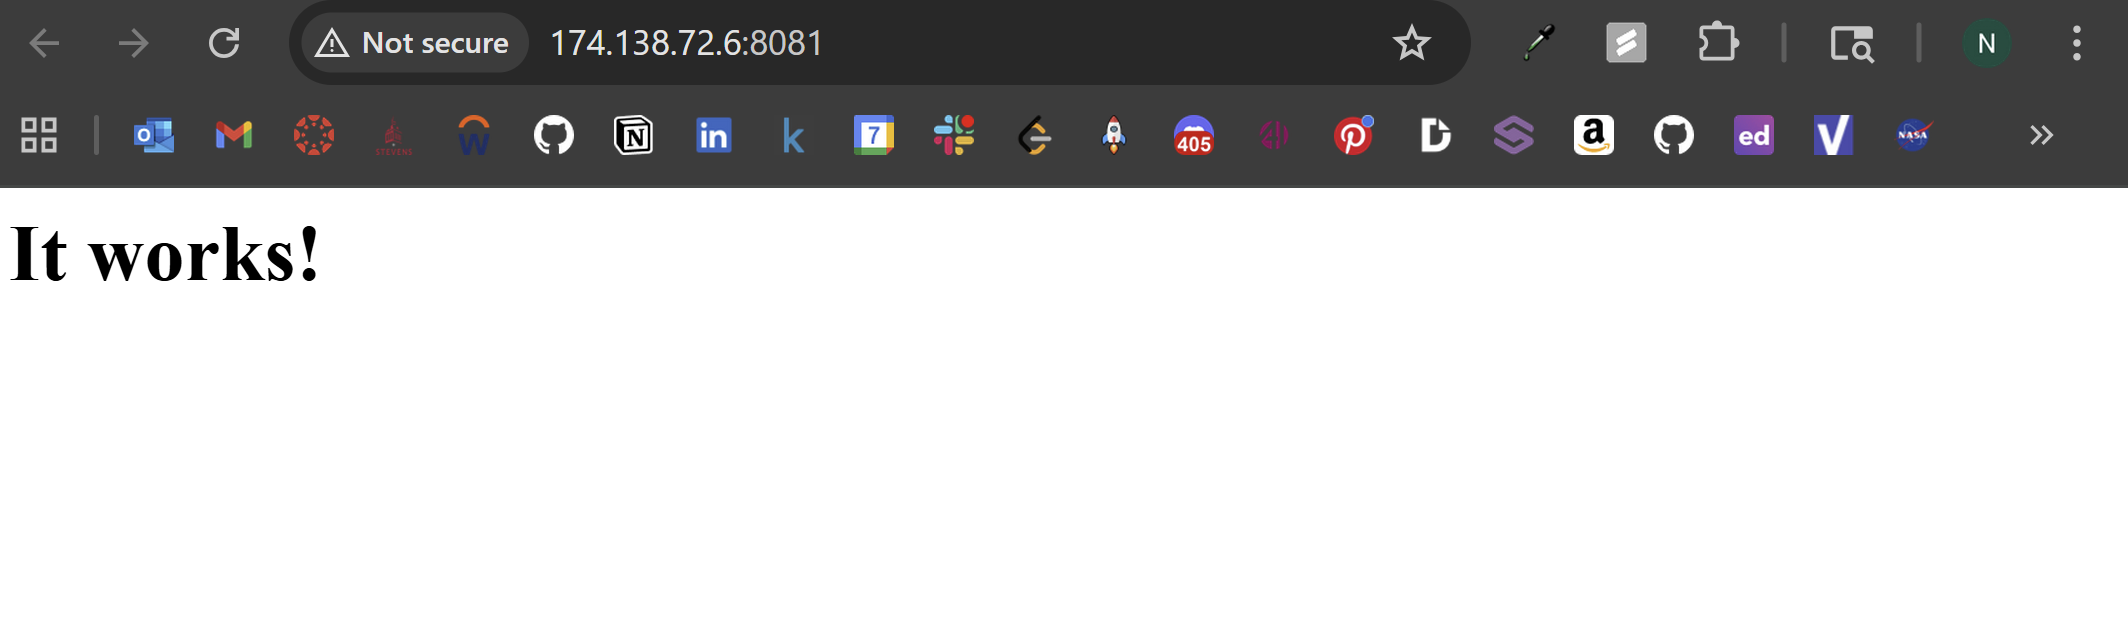
\includegraphics[width=0.6\linewidth]{Book_SSW590_1/eps/Screenshots/Overleaf_1.png}
    \caption{Working IP}
    \label{fig: Working IP}
\end{figure}


\begin{figure}[ht]
    \centering
    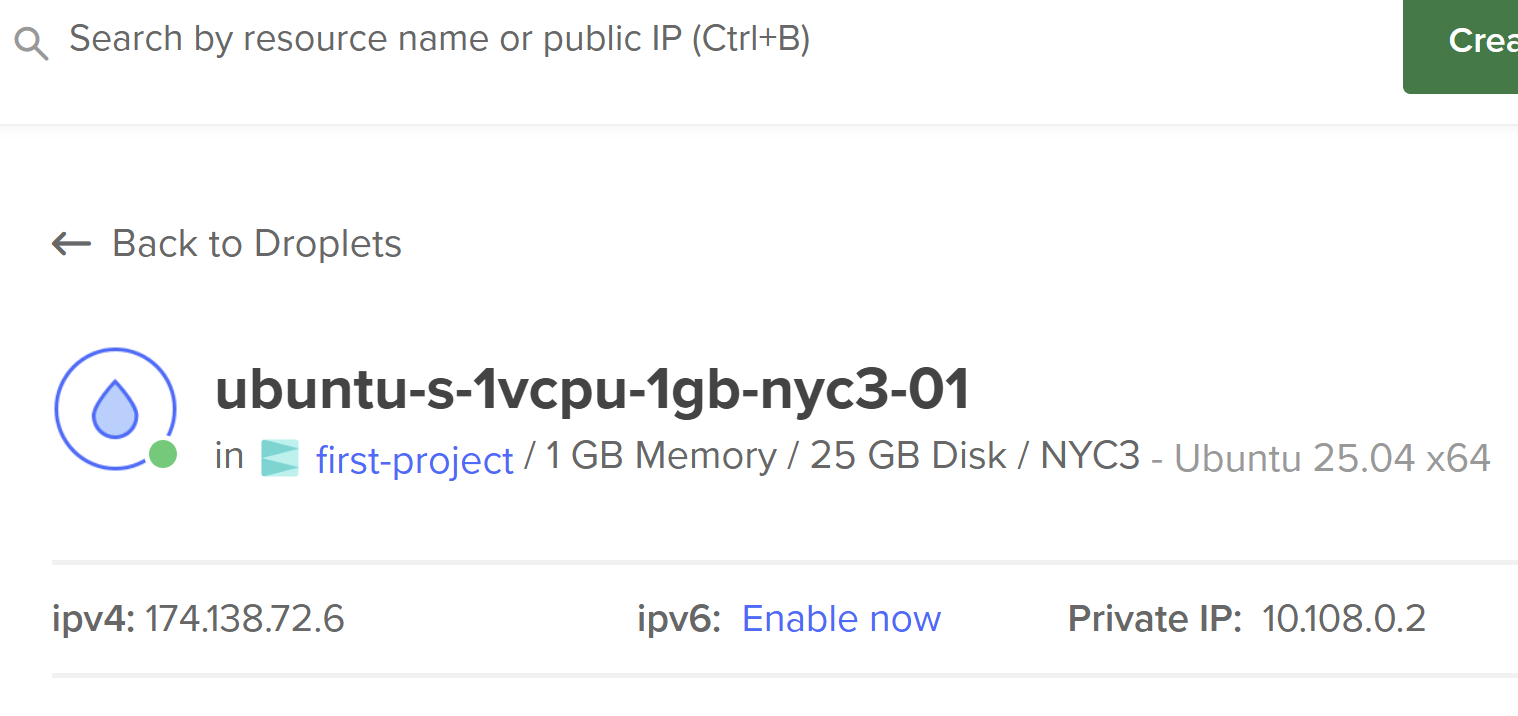
\includegraphics[width=0.6\linewidth]{Book_SSW590_1/eps/Screenshots/Overleaf_2.png}
    \caption{IP}
    \label{IP}
\end{figure}

\chapter{Overleaf \\
\small{\textit{-- Nataly Jimenez, Nicole Valdiviezo, Lakshya Vegiraju}}
\index{Overleaf} 
\index{Chapter!Overleaf}
\label{Chapter::Overleaf}}

\section{Overview}
Overleaf is an online collaborative \LaTeX{} editor that simplifies the writing and publishing of scientific documents. The team deployed it as a Docker container on a DigitalOcean Droplet using free credits from the GitHub Student Developer Pack. This setup provides full control, offline access, and integration with other self-hosted services, such as Bugzilla.

\section{SSH Using Droplet IP}
\begin{minted}{bash}
PS C:\Users\natnj> ssh root@104.248.14.71
root@ubuntu-s-1vcpu-512mb-10gb-nyc3-01:~# snap install docker
\end{minted}

\section{Pull and Run Overleaf Image}
\begin{minted}{bash}
docker run -d -p 8080:80 --name overleaf nginx
http://104.248.14.71:8080/
\end{minted}

\section{Screenshot from Browser}
The following screenshots provide evidence of assignment completion for the Bugzilla section of the project:

\begin{figure}[ht]
    \centering
    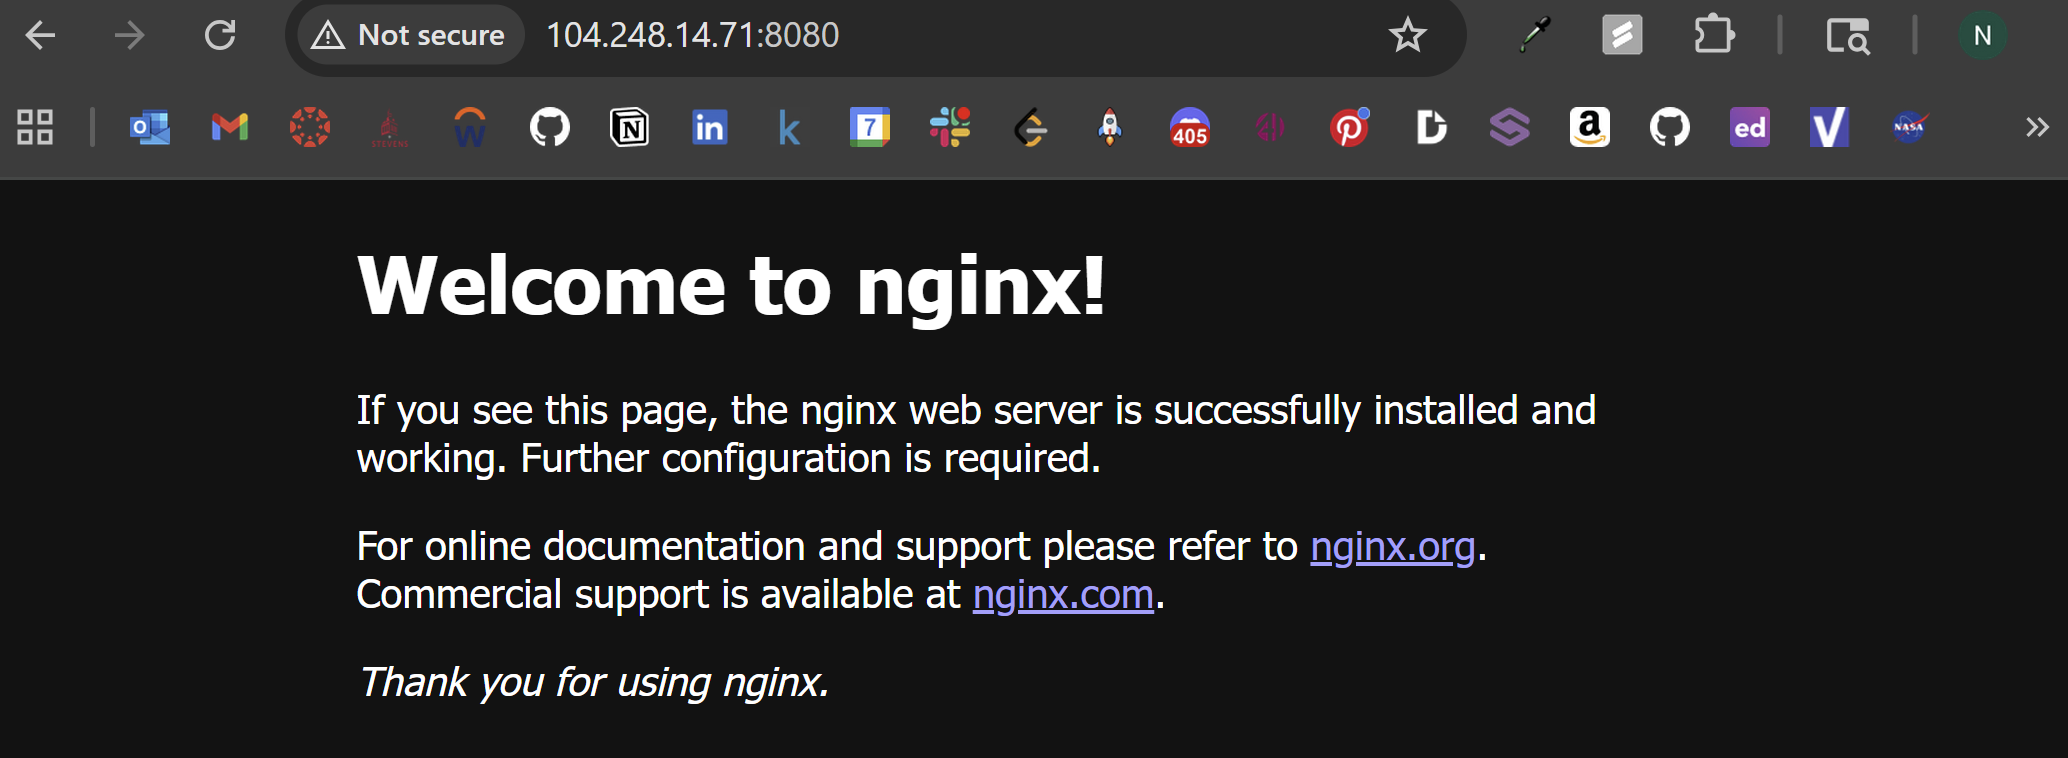
\includegraphics[width=0.6\linewidth]{Book_SSW590 (1)/eps/Screenshots/Overleaf_6.png}
    \caption{NGINX Page}
    \label{NGINX Page}
\end{figure}

\chapter{Domain and SSL Setup \\
\small{\textit{-- Nataly Jimenez, Nicole Valdiviezo, Lakshya Vegiraju}}
\index{Domain and SSL Setup} 
\index{Chapter!Domain and SSL Setup}
\label{Chapter::DomainSSL Setup}}

\section{Step 1: Domain Name Setup}

\subsection{Overview}
For this project, our group registered a custom domain name to host our Overleaf instance. We selected the domain \textbf{audioviz.me}, which was purchased through \textbf{Namecheap}. This domain will later be connected to our Overleaf container and GitHub repository for version-controlled LaTeX compilation and deployment.

\subsection{Procedure}
\begin{enumerate}
    \item \textbf{Domain Registration:}
    \begin{itemize}
        \item Visited \url{https://www.namecheap.com/} and searched for an available domain name.
        \item Registered the domain \textbf{audioviz.me} under our group’s Namecheap account.
        \item Verified ownership via the confirmation email sent by Namecheap.
    \end{itemize}

    \item \textbf{DNS Configuration:}
    \begin{itemize}
        \item Logged into the Namecheap dashboard.
        \item Navigated to \textit{Domain List → Manage → Advanced DNS}.
        \item Created an \textbf{A record} pointing to the IP address of our Overleaf server or cloud host (e.g., DigitalOcean, AWS, or local machine).
        \item Optionally, added a \textbf{CNAME record} for subdomains (e.g., \texttt{overleaf.audioviz.me}) pointing to the root domain.
        \item Saved changes and waited for DNS propagation (typically 10–30 minutes).
    \end{itemize}

    \item \textbf{Verification:}
    \begin{itemize}
        \item Used \texttt{nslookup audioviz.me} and \texttt{ping audioviz.me} to confirm DNS resolution.
        \item Accessed the domain in a browser to ensure it correctly routed to our host IP.
    \end{itemize}
\end{enumerate}

\subsection{Next Steps}
\begin{itemize}
    \item Configure Nginx or Apache as a reverse proxy for the Overleaf container.
    \item Ensure ports 80 (HTTP) and 443 (HTTPS) are open on the server.
\end{itemize}

\section{Step 2: SSL Configuration Research}

\subsection{Overview}
To secure our domain with HTTPS, we researched methods to add and renew SSL certificates for the Overleaf instance. The preferred approach uses \textbf{Let’s Encrypt}, a free Certificate Authority that automatically renews every 90 days.

\subsection{Installation and Renewal Options}
\begin{enumerate}
    \item \textbf{Install Certbot (Let’s Encrypt client):}
    \begin{verbatim}
    sudo apt update
    sudo apt install certbot python3-certbot-nginx
    \end{verbatim}

    \item \textbf{Obtain a Certificate:}
    \begin{verbatim}
    sudo certbot --nginx -d audioviz.me -d overleaf.audioviz.me
    \end{verbatim}
    This command:
    \begin{itemize}
        \item Automatically configures Nginx for SSL.
        \item Downloads and installs certificates for both the root and subdomain.
    \end{itemize}

    \item \textbf{Test Auto-Renewal:}
    \begin{verbatim}
    sudo certbot renew --dry-run
    \end{verbatim}

    \item \textbf{Alternative (Manual or Dockerized Setup):}
    \begin{itemize}
        \item If running Overleaf inside Docker, mount certificate volumes:
        \begin{verbatim}
        docker run -d \
            -v /etc/letsencrypt/live/audioviz.me:/etc/letsencrypt/live/audioviz.me \
            -p 80:80 -p 443:443 \
            overleaf/overleaf
        \end{verbatim}
        \item Configure the Overleaf container to use SSL via the Nginx proxy container.
    \end{itemize}
\end{enumerate}

\subsection{Next Steps}
\begin{itemize}
    \item Integrate SSL configuration into the Overleaf Docker Compose file.
    \item Set up a cron job or systemd timer for automatic certificate renewal.
    \item Update the documentation with screenshots of the SSL verification (using \texttt{https://audioviz.me}).
\end{itemize}

\subsection{Install Docker and Docker Compose on droplet}

\begin{minted}{bash}
# Update system
sudo apt update && sudo apt upgrade -y

# Install Docker
curl -fsSL https://get.docker.com -o get-docker.sh
sudo sh get-docker.sh

# Install Docker Compose
sudo apt install docker-compose -y

# Add current user to Docker group
sudo usermod -aG docker $USER

\end{minted}

\section{Summary}
After completing Steps 1 and 2, the group will have:
\begin{itemize}
    \item A working domain \textbf{(audioviz.me)} that points to the Overleaf host.
    \item A secure HTTPS connection via Let’s Encrypt.
    \item A foundation to connect Overleaf with GitHub and compile LaTeX projects under version control.
\end{itemize}



\section{Step 3: Set up Overleaf container}
\begin{minted}{bash}
mkdir -p ~/overleaf
cd ~/overleaf
\end{minted}

\begin{minted}{bash}
nano docker-compose.yml
\end{minted}

\begin{minted}{bash}
version: '3.8'

services:
  overleaf:
    image: sharelatex/sharelatex:latest
    restart: always                   # Restarts if container crashes or droplet reboots
    ports:
      - "80:80"                       # Exposes HTTP
      - "443:443"                     # Exposes HTTPS (for SSL)
    environment:
      - ROOT_URL=https://audioviz.me  # The domain Overleaf will use
    volumes:
      - ./data:/var/lib/sharelatex
    -./tmp:/var/lib/sharelatex/tmp
      - /var/run/docker.sock:/var/run/docker.sock
\end{minted}

\begin{minted}{bash}
docker-compose pull
docker-compose up -d
\end{minted}

\subsection{Configure Overleaf Container}
\begin{itemize}
  \item Set up a custom Overleaf container using the latest LaTeX image with all required packages preinstalled.
  \item Installed additional packages (\texttt{biblatex}, \texttt{tikz}, \texttt{geometry}, and \texttt{hyperref}) to support group document formatting.
  \item Verified compilation by building our main \texttt{.tex} project 
  \item Adjusted the Dockerfile to ensure consistent LaTeX builds across all group members.
  \item Noted configuration details and build success in our update log.
\end{itemize}

\section{Step 4 – Connect Overleaf to GitHub}
\begin{itemize}
  \item Created a private GitHub repository for our Overleaf project and initialized it with a \texttt{README.md}.
  \item Linked Overleaf to the repository via the built-in GitHub integration.
  \item Pushed our project to GitHub and confirmed that all files (\texttt{.tex}, images, and \texttt{.bib}) synced correctly.
  \item Tested syncing in both directions 
  \item Documented connection steps and repository link in our update history table.
\end{itemize}

\section{Step 5 – Compile from Command Line}
\begin{itemize}
  \item Cloned the GitHub repository locally using the command:
  \begin{verbatim}
  git clone https://github.com/yourusername/yourproject.git
  \end{verbatim}

  \item Navigated into the project directory:
  \begin{verbatim}
  cd yourproject
  \end{verbatim}

  \item Compiled the LaTeX document with the following commands to ensure reproducible builds:
  \begin{verbatim}
  latexmk -pdf main.tex
  \end{verbatim}
  or alternatively:
  \begin{verbatim}
  pdflatex main.tex
  bibtex main.aux
  pdflatex main.tex
  pdflatex main.tex
  \end{verbatim}

  \item Installed missing LaTeX dependencies as needed:
  \begin{verbatim}
  tlmgr install <package-name>
  \end{verbatim}

  \item Verified that the compiled PDF matched Overleaf’s online output and noted any differences.
\end{itemize}

\section{Step 6 – Add Versioning to the Project}
\begin{itemize}
  \item Added the version number and the short Git commit hash on the document title page.
  \item Confirmed version traceability by cross-checking GitHub tags with Overleaf project history.
\end{itemize}



\appendix
\chapter{Appendix \\
\small{\textit{-- Nataly Jimenez, Nicole Valdiviezo, Lakshya Vegiraju}}
\index{appendix} 
\index{Chapter!Appendix}
\label{Chapter::Appendix}}

% makeglossaries dsnManual -- from command prompt.
\clearpage
%\printglossaries


\printnoidxglossaries

\bibliography{bibfile}
%\bibliographystyle{unsrt}
\bibliographystyle{IEEEtran}

\printindex
%\input{dsnManual.idx}
\end{document}
